%\documentclass[a4paper,12pt]{book}
\documentclass[a4paper,12pt]{report}
%\usepackage{mathpazo}
\usepackage{amsmath} % จะใช้ package ของ math อื่นใด ให้เรียกก่อน fontspec
\usepackage{amssymb} % จะใช้ package ของ math อื่นใด ให้เรียกก่อน fontspec
\usepackage{amsfonts} % จะใช้ package ของ math อื่นใด ให้เรียกก่อน fontspec
\usepackage{mathspec} % เรียกใช้แค่นี้มีค่า = \usepackage[no-math]{fontspec}\usepackage{mathspec}
\usepackage{xunicode,xltxtra}
\XeTeXlinebreaklocale "th"
\XeTeXlinebreakskip = 0pt plus 1pt %
\defaultfontfeatures{Scale=1.23}
\renewcommand{\baselinestretch}{1.2}
\setmainfont{TH Sarabun New}
\newfontfamily\kodchasal{TH Kodchasal} % ตั้งชื่อฟอนต์ใหม่เพื่อให้ง่ายต่อการใช้งาน เผื่อว่าในเอกสารต้องการให้มีหลายฟอนต์ เวลาใช้ก็ {\examplefont ข้อความต่าง ๆ}
\newfontfamily\niramit{TH Niramit AS}
\usepackage{xcolor}
\definecolor{MyColor}{rgb}{0.3,0.4,0.5} % กำหนดสี และชื่อที่จะใช้เรียกสีโดย xcolor
\everymath{\displaystyle} % บังคับให้ทุกสมการเป็น displaystyle
\usepackage{tabls}
\usepackage{graphicx}
\usepackage{tabularx}
\usepackage{booktabs}
\usepackage{longtable}
\usepackage{wrapfig} %ตัวหนังสือล้อมรอบรูปหรือตารางได้ (wrapfigure,wraptable) *** ไม่สามารถอยู่ในพวก enumerate ได้
\usepackage[Glenn]{fncychap}
\usepackage{sectsty,ulem}
\allsectionsfont{\ulemheading{\uline}}
\makeatletter
\def\@seccntformat#1{\csname the#1\endcsname)\quad}
\makeatother
\usepackage{cellspace}
\usepackage[usenames,dvipsnames]{pstricks} 
\usepackage{epsfig} 
\usepackage{pst-grad} % For gradients
\usepackage{pst-plot} % For axes 
\usepackage{makecell}
\usepackage{fancyhdr}
\usepackage{lastpage}
\usepackage{fancybox}
\usepackage{multirow}
\usepackage{calc}
% ระยะช่องว่างหน้า+หลังเลขหรืออักษรในสมการ หน่วยเป็น mmu , 1 mmu = 1mu/1000 , 18mu = 1 em ,default = 500 mmu = 1/36 em 
% ตัวไหนจะให้มีระยะพิเศษก็ใส่ " นำหน้า เช่น $ x^{"2} หรือใส่ทีละคำให้ใส่เป็น $ x^{\"3yz"} $
% \setminwhitespace[XXXX] 
\setminwhitespace[3000] 

% เลือก Math Font ต่าง ๆ นา ๆ
%\setmathsfont(Digits,Latin){Asana Math}
%\setmathsfont(Digits,Latin){jsMath-cmr10}
%\setmathsfont(Digits,Latin){Kerkis}
%\setmathsfont(Digits,Latin){Neo Euler}
%\setmathsfont(Digits,Latin){Fontin}
%\setmathsfont(Digits,Latin){Plakken}
%\setmathsfont(Digits,Latin){DejaVu Serif}
%\setmathsfont(Digits,Latin){STIXGeneral}
%\setmathsfont(Digits,Latin){CMU Bright}
%\setmathsfont(Digits,Latin){Iwona Light}
%\setmathsfont(Digits,Latin,Greek)[Numbers={Lining,Proportional}]{Iwona Light}
%\setmathsfont(Digits,Latin,Greek){TH Sarabun New}
%\setmathsfont(Digits,Latin,Greek){Mathmos Original}
% ใช้ฟอนต์ OTF ในเอกสารแต่ MATH ใช้ฟอนต์ Math
%\usepackage[no-math]{fontspec}

% ใช้ฟอนต์ OTF ในเอกสารและ MATH ใช้ฟอนต์ OTF
%\usepackage[no-math]{fontspec}
%\usepackage{mathspec}
%\setmainfont{TH Sarabun New}
%\setallmainfonts(Digits,Latin,Greek){TH Sarabun New}
\setallmainfonts(Digits,Latin,Greek){TH Sarabun New}

% \setmathrm จะเปลี่ยนฟอนต์เฉพาะที่อยู่ในคำสั่ง \mathrm{.....} เท่านั้น
%\setmathrm{TH Sarabun New}
%\setmathsfont(Digits,Latin,Greek){TH Sarabun New}
%\setmathfont(Digits,Latin,Greek){TH Sarabun New}

\pagestyle{fancy}
\fancyhead[L]{ติวสบายฟิสิกส์}
\fancyhead[R]{www.pec9.com}
% ------- เอารูปวางตรงไหนก็ได้ในเอกสาร ---------
% ------- ใช้ทำเส้นข้างร่วมกับ fancyhdr ----------
\usepackage{eso-pic,picture}
\usepackage[absolute]{textpos}
    \setlength{\TPHorizModule}{10mm}% 1 generic horizontal unit is equivalent to 10mm
    \setlength{\TPVertModule}{10mm}% 1 generic vertical unit is equivalent to 10mm
    \textblockorigin{0mm}{0mm}% top left corner set as origin
\newcommand{\mytikz}{\tikz \draw (0,0)--(0,-20);}
\fancyfoot[LO]{ \begin{textblock}{3}(17,2) \mytikz \end{textblock} }
\fancyfoot[RE]{ \begin{textblock}{3}(1.1,2) \mytikz \end{textblock} }
% ----------------- จบ ---------------------
%\setlist[enumerate,1]{leftmargin=*,resume} % ตั้งให้ enumerate level 1 ไม่ indent และต่อข้ออัตโนมัติ โดยไม่ต้องใช้ counter
\begin{document}
%\mainmatter % สำหรับ book
\chapter{การเคลื่อนที่}
\section{การเคลื่อนที่แนวตรง}
\begin{c2}		\subsection{ระยะทาง การกระจัด อัตราเร็ว และความเร็ว}
		\begin{minipage}{\textwidth}
			\begin{tabbing}
				\textbf{ระยะทาง} \quad \=\textbf{คือ} ความยาวตามแนวที่เคลื่อนที่ได้จริง มีหน่วยเป็นเมตร (m) \\
				\textbf{การกระจัด} 		\>\textbf{คือ} \=ความยาวที่วัดเป็นเส้นตรงจากจุดเริ่มต้นถึงจุดสุดท้ายของ\\
														\>\>การเคลื่อนที่มีหน่วยเป็นเมตร (m)
			\end{tabbing}
			\adjustbox{valign=t}{
				\begin{minipage}[t]{0.6\linewidth}
					\textbf{ตัวอย่างเช่น} หากวัตถุก้อนหนึ่งเคลื่อนที่จากจุด A  ไปจุด B  แล้วเคลื่อนต่อไปจุด C  ในทิศที่ตั้งฉากกันดังรูป   จะได้ว่า	
					\begin{align*}
						\text{ระยะทาง} &= \text{ตามแนวที่เคลื่อนที่ได้จริง} \\
						\text{ระยะทาง} &= 4 + 3 \text{เมตร} \\
						\text{ระยะทาง} &= 7 \text{เมตร}	\quad \text{\textbf{*** ไม่ต้องสนใจทิศทาง}}
					\end{align*}
				\end{minipage}
			}%
			\hfill
			\adjustbox{valign=t}{
				\begin{minipage}[t]{0.3\linewidth}
	    			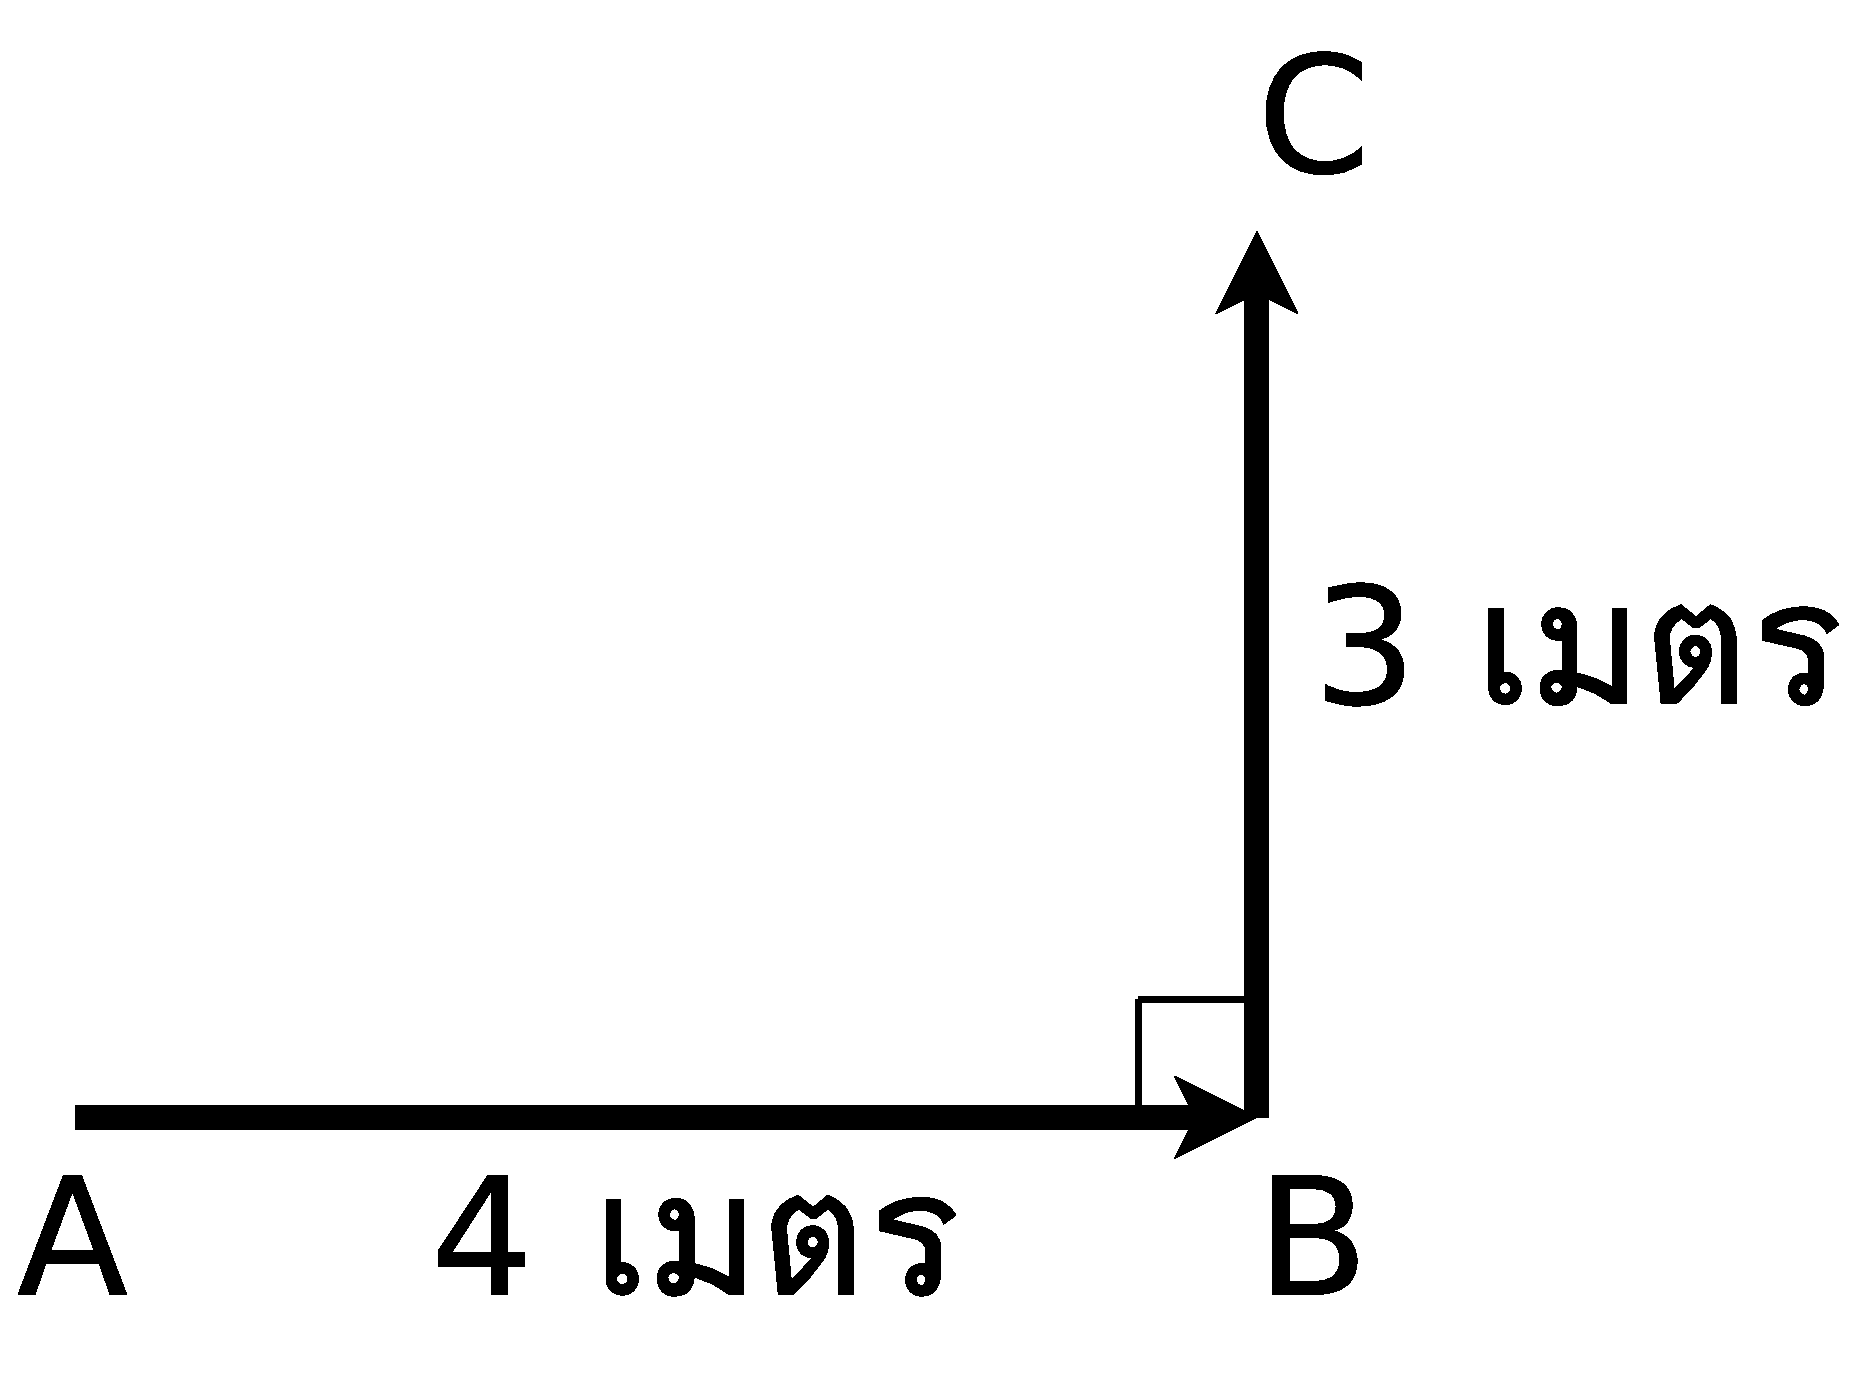
\includegraphics[width=\linewidth]{pic1.eps}
				\end{minipage}
			}
		\end{minipage}
		\begin{minipage}{\textwidth}
					\textbf{และจะได้อีกว่า}\\
			\adjustbox{valign=t}{
				\begin{minipage}[t]{0.6\linewidth}
					\begin{tabbing}
						การกระจัด \= $=$ \=ความยาวที่วัดเป็น\underline{เส้นตรง}จาก \\
									\>\>จุดเริ่มต้นถึงจุดสุดท้าย \\
						การกระจัด \> $=$ 5  \text{เมตร} 
					\end{tabbing}
				\end{minipage}
			}%
			\hfill
			\adjustbox{valign=t}{
				\begin{minipage}[t]{0.3\linewidth}
	    			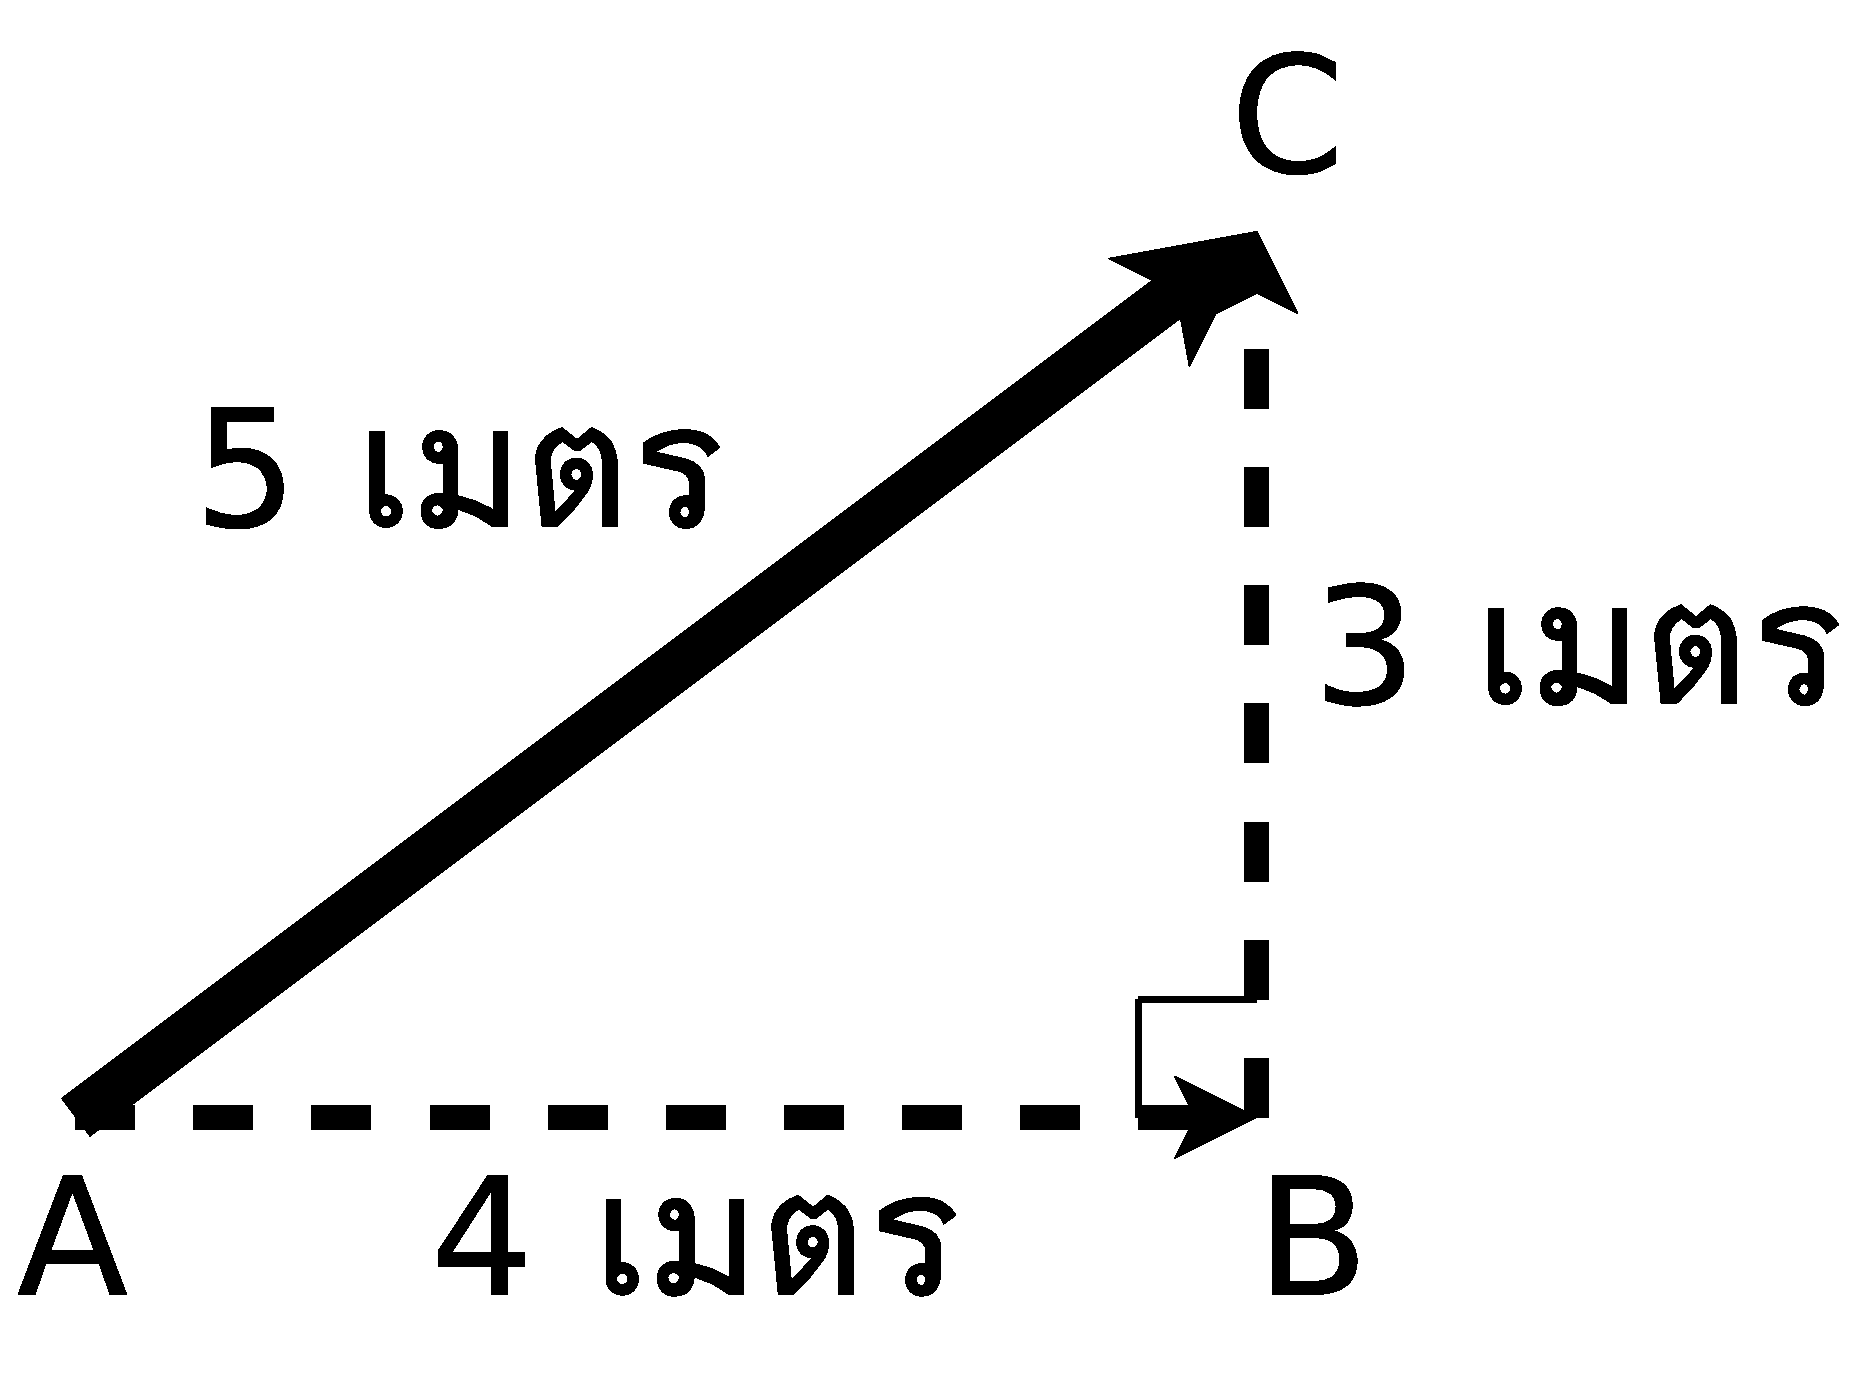
\includegraphics[width=\linewidth]{pic2.eps}
				\end{minipage}
			}	
			\begin{center}
				\textbf{*** การกระจัดนี้มีทิศจากจุดเริ่มต้น (A) ไปถึงจุดสุดท้าย (C)}
			\end{center}
		\end{minipage}
\end{c2}
\begin{enumerate}
\item   \begin{ljrp} 
            ระยะทางและการกระจัดของการเคลื่อนที่ต่อไปนี้ มีขนาดเท่ากับกี่เมตรตามลําดับ \runningj
            \begin{4c}
                {12,8}{8,10}{8,12}{10,8}
            \end{4c}
        \end{ljrp}
        \begin{rp}{pic-jote-1.eps}\end{rp}
\end{enumerate}

\begin{enumerate}
	\item  \runningj \nonet  คลองที่ตัดตรงจากเมือง  A  ไปเมือง  B  มีความยาว  72  กิโลเมตร  ขณะที่ถนนคดเคี้ยวจากเมือง  A  ไปเมือง  B  มีความยาว  83  กิโลเมตร  ถ้าชายคนหนึ่งขนสินค้าจากเมือง  A  ไปเมือง  B  โดยรถยนต์  ถามว่าการเคลื่อนที่ครั้งนี้มีขนาดการกระจัดเท่าใด 
	\begin{4c}
		{11 km}{65 km}{72 km}{83 km}
	\end{4c}
\end{enumerate}

\begin{enumerate}
	\item  \nonet  วัตถุหนึ่งเคลื่อนที่เป็นวงกลมรัศมี   14  เมตรครบหนึ่งรอบ   การกระจัดมีค่าเท่าใด \runningj
	\begin{4c}
		{0 เมตร}{14 เมตร}{44 เมตร}{88 เมตร}
	\end{4c}
\end{enumerate}

\begin{c2}	\textbf{อัตราเร็วเฉลี่ย} หาค่าได้จากอัตราส่วนระหว่างระยะทางที่เคลื่อนที่ได้กับเวลาที่ในการเคลื่อนที่ช่วงนั้น  มีหน่วยเป็นเมตรต่อวินาที ( m/s ) \textbf{นั่นคือ}
				$$        \text{อัตราเร็วเฉลี่ย}  =  \frac{\text{ระยะทางที่เคลื่อนที่ได้}}{\text{เวลาที่ใช้}} $$ 
	\textbf{ความเร็วเฉลี่ย} หาค่าได้จากอัตราส่วนระหว่างการกระจัดของเคลื่อนที่กับเวลาที่ในการเคลื่อนที่ช่วงนั้น  มีหน่วยเป็นเมตรต่อวินาที ( m/s ) \textbf{นั่นคือ}
				$$        \text{ความเร็วเฉลี่ย}  =  \frac{\text{การกระจัด}}{\text{เวลาที่ใช้}} $$
\end{c2}
\begin{enumerate}
	\item \runningj  \nonet เด็กคนหนึงวิงเป็นเส้นตรงไปทางขวา 10 เมตร ในเวลา 3 วินาที จากนันหันกลับแล้ววิ่งเป็นเส้นตรงไปทางซ้ายอีก 5 เมตร ในเวลา 2 วินาที อัตราเร็วเฉลี่ยของเด็กคนนีเป็นไปตามข้อใด 
	\begin{2c}
		{1.0 เมตรต่อวินาท}{3.0 เมตรต่อวินาท}{5.0 เมตรต่อวินาท}{7.5 เมตรต่อวินาท}
	\end{2c}
\end{enumerate}

\begin{enumerate}
	\item \runningj  \nonet จากข้อที่ผ่านมา  ขนาดของความเร็วเฉลี่ยของเด็กคนนี้เป็นไปตามข้อใด
	\begin{2c}
		{1.0  เมตรต่อวินาที}{3.0  เมตรต่อวินาที}{5.0  เมตรต่อวินาที}{7.5  เมตรต่อวินาที}
	\end{2c}
\end{enumerate}

\begin{enumerate}
	\item \runningj  \nonet เด็กคนหนึ่งเดินไปทางทิศตะวันออกได้ระยะทาง  40  เมตร  จากนั้นเดินไปทางทิศเหนือได้ระยะทาง  30  เมตร  ใช้เวลาเดินทางทั้งหมด  100  วินาที  เด็กคนนี้เดินด้วยอัตราเร็วเฉลี่ยกี่เมตร/วินาที 
	\begin{2c}
		{0.5 m/s}{0.7 m/s}{1.0 m/s}{1.4 m/s}
	\end{2c}
\end{enumerate}

\begin{enumerate}
	\item \runningj  \nonet ตอนเริ่มต้นวัตถุอยู่ห่างจากจุดอ้างอิงไปทางขวา  2.0  เมตร   เมื่อเวลาผ่านไป  10  	วินาที   พบว่าวัตถุอยู่ห่างจากจุดอ้างอิงไปทางซ้าย   3.0  เมตร  จงหาความเร็วเฉลี่ยของวัตถุนี้ 
	\begin{2c}
		{0.5  เมตรต่อวินาที 	 ทางขวา}{0.5  เมตรต่อวินาที  ทางซ้าย}{1.0  เมตรต่อวินาที 	 ทางขวา}{1.0  เมตรต่อวินาที  ทางซ้าย}
	\end{2c}
\end{enumerate}

\begin{enumerate}
	\item \ncmu รถโดยสารเริ่มออกเดินทางจากกรุงเทพฯ  เวลา   22.00  น.   มาถึงเชียงใหม่เวลา    	8.00 น.   กำหนดให้ระยะทางจากกรุงเทพฯถึงเชียงใหม่เป็น   720  กิโลเมตร   จงหาว่ารถโดยสารคันนี้วิ่งด้วยอัตราเร็วเฉลี่ยเท่าใด \runningj
	\begin{2c}
		{10  กิโลเมตรต่อชั่วโมง}{100  กิโลเมตรต่อชั่วโมง}{72  กิโลเมตรต่อชั่วโมง}{720  กิโลเมตรต่อชั่วโมง}
	\end{2c}
\end{enumerate}

\begin{c2}            กรณีที่วัตถุเคลื่อนที่ไปด้วยความเร็วคงที่   จะได้ว่า 
            \begin{align*} % ให้เครื่องหมาย = ในสมการเท่ากัน และไม่มีเลขกำกับสมการ
                \text{ระยะทางที่เคลื่อนที่ได้}  &=  \text{อัตราเร็ว}\times \text{เวลาที่ใช้เคลื่อนที่} \\
                \text{\textbf{หรือ}}\qquad \qquad              s  &=  v \cdot  t
            \end{align*}
            \begin{tabbing}
                    \textbf{เมื่อ} \quad  \=\textbf{s}  คือระยะทางที่เคลื่อนที่ได้ \quad \=หน่วยเป็นเมตร ( m ) \\
                                        \>\textbf{v}  คืออัตราเร็วซึ่งคงที่  \> หน่วยเป็นเมตรต่อวินาที ( m/s ) \\
                                        \>\textbf{t}  คือเวลาที่ใช้เคลื่อนที่  \> หน่วยเป็นวินาที ( s ) 
            \end{tabbing}
\end{c2}
\begin{enumerate}
	\item \runningj รถยนต์คันหนึ่งวิ่งด้วยอัตราเร็วคงตัว   15  เมตรต่อวินาทีเป็นเวลานาน  60  วินาที  	ระยะทางที่รถยนต์คันนี้เคลื่อนที่ได้จะมีขนาดเท่ากับข้อใดต่อไปนี้
	\begin{4c}
		{45 m}{90 m}{450 m}{900 m}
	\end{4c}
\end{enumerate}

\begin{enumerate}
	\item \runningj \nonet รถยนต์คันหนึ่งวิ่งด้วยอัตราเร็วคงตัว   15  เมตรต่อวินาที    นานเท่าใดจึงจะเคลื่อนที่ได้ระยะทาง  450  เมตร
	\begin{4c}
		{10 s}{15 s}{30 s }{45 s}
	\end{4c}
\end{enumerate}

\begin{c2}\subsection{ความเร่ง}
\textbf{ความเร่ง คือ} ความเร็วที่เปลี่ยนไปในหนึ่งหน่วยเวลา
\begin{align*}
	\text{\textbf{หาค่าได้จาก}} \qquad \text{ความเร่ง} &= \frac{\text{ความเร็วที่เปลี่ยนไป}}{\text{เวลาที่ใช้}} \\
							\text{ความเร่ง} &= \frac{\text{ความเร็วปลาย}-\text{ความเร็วต้น}}{\text{เวลาที่ใช้}} \\
	\text{\textbf{หรือ}} \qquad \qquad \qquad a &= \frac{v_2-v_1}{t}
\end{align*}
\begin{tabbing}
\textbf{เมื่อ} \quad	\=a		\quad \= คือความเร่ง		\quad\quad \= มีหน่วยเป็นเมตรต่อวินาที$^2$ (m/s$^2$) \\
					\>$v_1$	\quad \> คือความเร็วต้น 	\quad\quad \> มีหน่วยเป็นเมตรต่อวินาที (m/s) \\
					\>$v_2$	\quad \> คือความเร็วปลาย 	\quad\quad \> มีหน่วยเป็นเมตรต่อวินาที (m/s) \\
					\>t		\quad \> คือเวลาที่ใช้ 		\quad\quad \> มีหน่วยเป็นวินาที ( s )
\end{tabbing}
\end{c2}
\begin{enumerate}
	\item \runningj \nonet รถยนต์คันหนึ่งเคลื่อนที่จากหยุดนิ่งไปบนเส้นทางตรง  เวลาผ่านไป  10  วินาที  	มีความเร็วเป็น  25  เมตร/วินาที     ถ้าอัตราเร็วเพิ่มขึ้นอย่างสม่ำเสมอ   รถยนต์คันนี้มีความเร่งเท่าใด
	\begin{4c}
		{2.0 $m/s^2$}{2.5 $m/s^2$}{4.0 $m/s^2$}{5.0 $m/s^2$}
	\end{4c}
\end{enumerate}

\begin{enumerate}
	\item \runningj เด็กคนหนึ่งวิ่งตรงไปด้วยความเร่ง   3  เมตรต่อวินาที$^2$    ถ้าเขาเริ่มต้นวิ่งจากหยุดนิ่ง  อีก  	10  วินาทีต่อมา   เขาจะมีความเร็วเท่าใด
	\begin{4c}
		{2 m/s}{10 m/s}{15 m/s}{30 m/s}
	\end{4c}
\end{enumerate}

\begin{c2}\textbf{ควรทราบ}
\begin{tabbing}
\quad 	\=$\blacktriangleright $ถ้าความเร่ง (a) มีค่าเป็น\textbf{บวก}	จะทำให้ความเร็ว (v) ของการเคลื่อนที่มีค่าเพิ่มขึ้น \\
		\>$\blacktriangleright $ถ้าความเร่ง (a) \=มีค่าเป็น\textbf{ลบ}  \underline{(อาจเรียกอีกอย่างว่าความหน่วง)}  จะทำให้ความเร็ว (v) \\
		\>\>ของการเคลื่อนที่มีค่าลดลง \\
		\>$\blacktriangleright $ถ้าความเร่ง (a) มีค่าเป็น\textbf{ศูนย์}  จะทำให้ความเร็ว (v) ของการเคลื่อนที่คงที่
\end{tabbing}
\end{c2}
\begin{enumerate}
\item \runningj \nonet ในการเคลื่อนที่เป็นเส้นตรง  กราฟข้อใดแสดงว่าวัตถุเคลื่อนที่ด้วยความเร็วคงตัว
	\begin{4c}
		{\begin{adjustbox}{valign=t}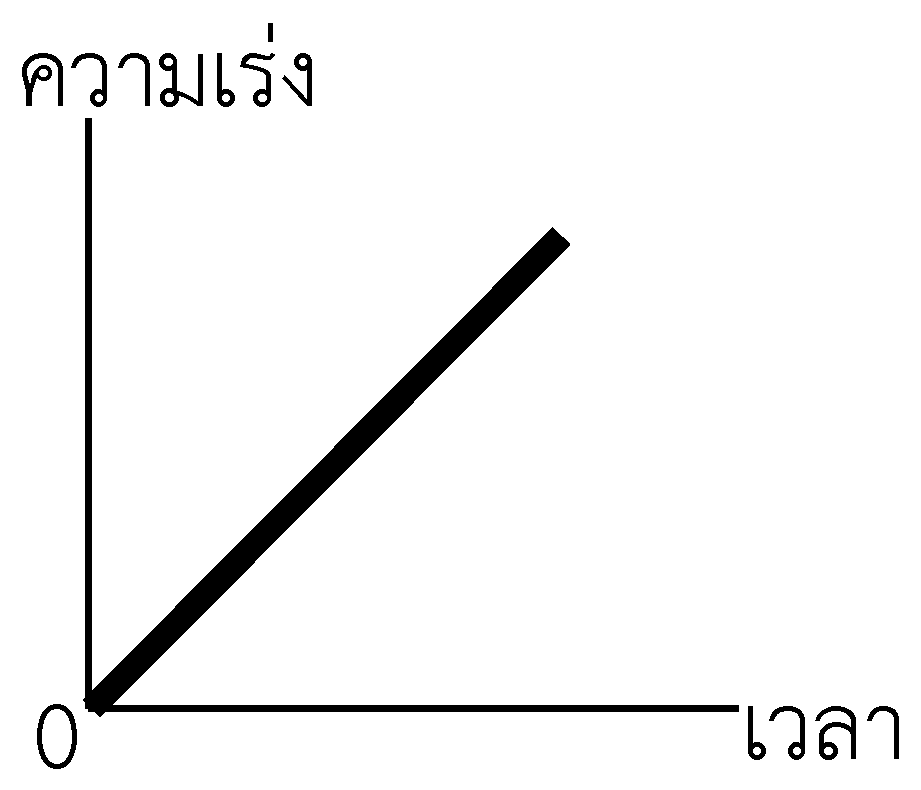
\includegraphics[width=\linewidth]{pic-17-1.pdf}\end{adjustbox}}
		{\begin{adjustbox}{valign=t}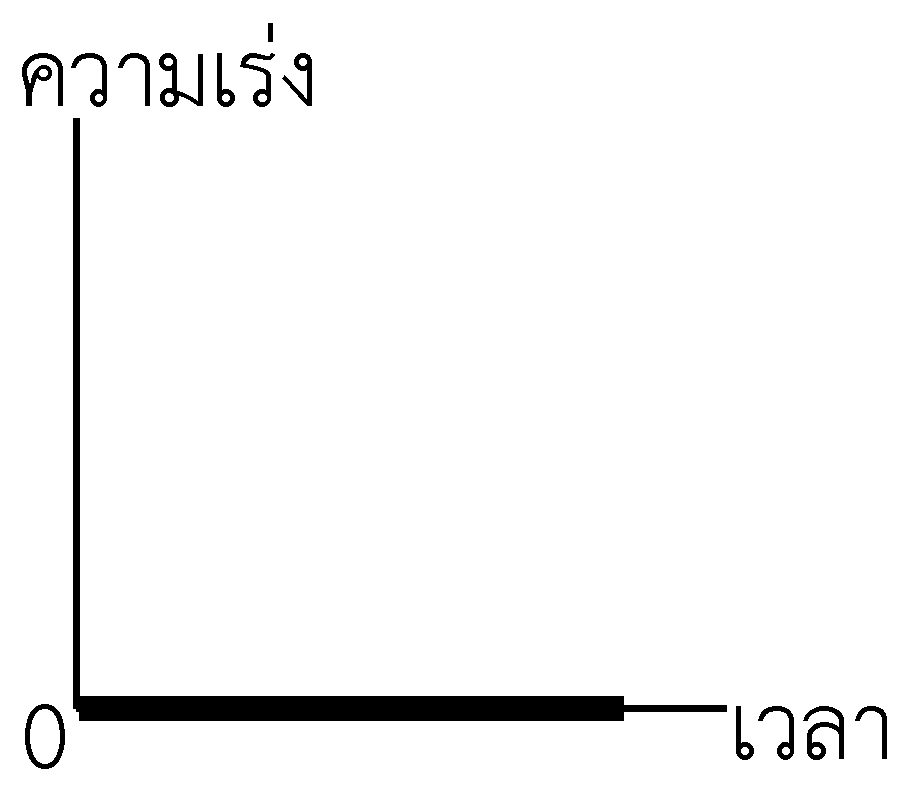
\includegraphics[width=\linewidth]{pic-17-2.pdf}\end{adjustbox}}
		{\begin{adjustbox}{valign=t}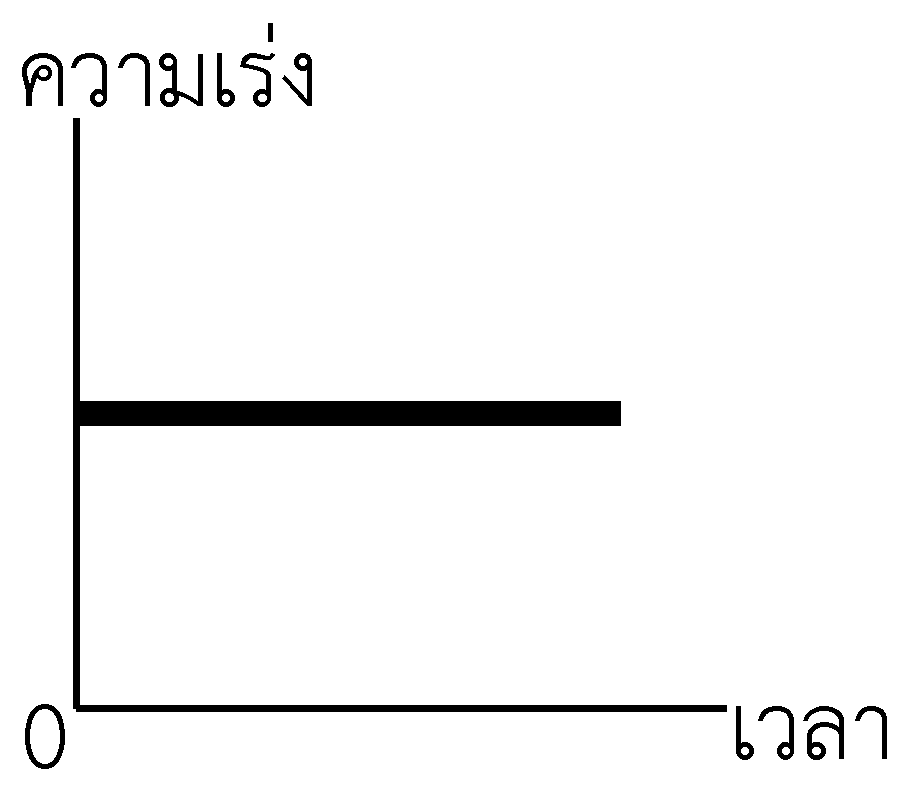
\includegraphics[width=\linewidth]{pic-17-3.pdf}\end{adjustbox}}
		{\begin{adjustbox}{valign=t}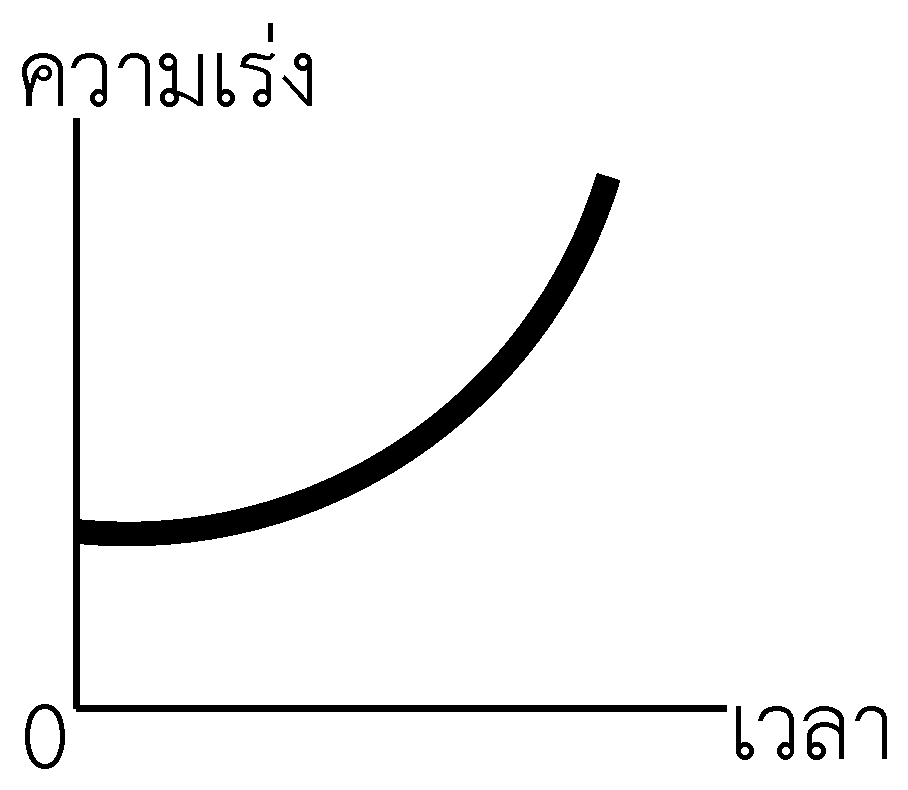
\includegraphics[width=\linewidth]{pic-17-4.pdf}\end{adjustbox}}
	\end{4c} 
\end{enumerate}

\begin{c2}\textbf{เกี่ยวกับการเคลื่อนที่เป็นเส้นตรงในแนวดิ่ง}
\tcblower 
\begin{minipage}{0.6\linewidth}
ขณะวัตถุเคลื่อนที่ในแนวดิ่งวัตถุจะถูกแรงดึงดูดของโลกดูดเอาไว้  ทำให้เกิดความเร่งเนื่องจากแรงโน้มถ่วงในทิศพุ่งลงสู่พื้นโลก \hfill และมีขนาดประมาณ  \\ 9.8  เมตร/วินาที$^2$  ความเร่งนี้นิยมใช้สัญลักษณ์แทนด้วย  g
\end{minipage}\hfill
\begin{adjustbox}{valign=c} \begin{minipage}[t]{.35\linewidth}
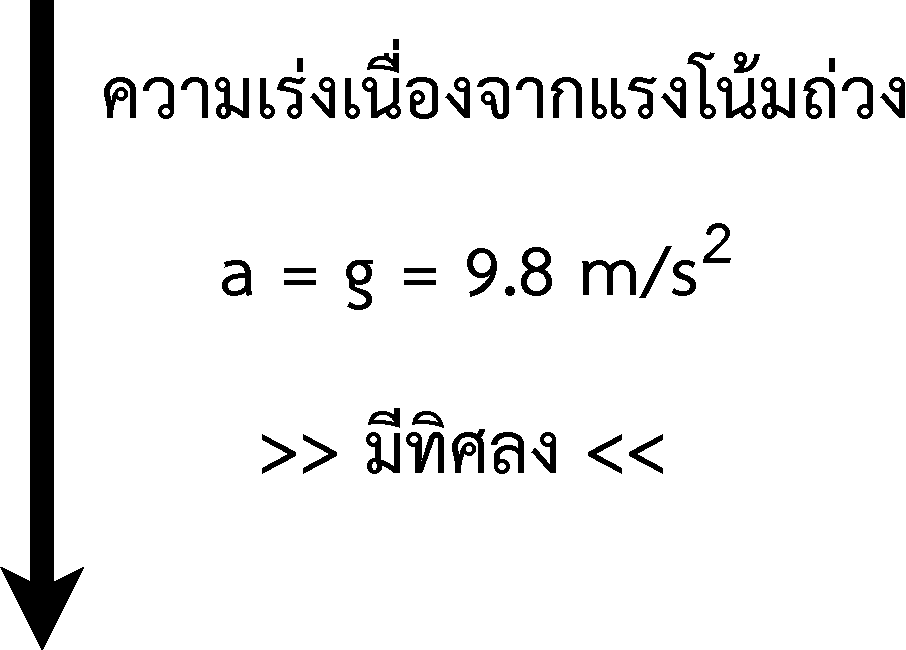
\includegraphics[width=\linewidth]{content-6.pdf}
\end{minipage}
\end{adjustbox}
\end{c2}
\begin{enumerate}
	\item \runningj \nonet ปล่อยวัตถุให้ตกลงมาตามแนวดิ่ง  เมื่อเวลาผ่านไป  6  วินาที  วัตถุมีความเร่งเท่าใด
	\begin{2c}
		{9.8 เมตรต่อวินาที$^2$}{19.6 เมตรต่อวินาที$^2$}
		{29.4 เมตรต่อวินาที$^2$}{39.2 เมตรต่อวินาที$^2$}
	\end{2c}
\end{enumerate}

\begin{enumerate}
\item \runningj \cmu{53} เมื่อโยนลูกเทนนิสขึ้นในแนวดิ่ง  ถ้าไม่คิดแรงต้านของอากาศ  ความเร่งของลูกเทนนิสจะมีทิศเข้าสู่ศูนย์กลางของโลกเมื่อใดบ้าง \\
	ก. เมื่อลูกเทนนิสกำลังเคลื่อนที่ขึ้น \\
	ข. เมื่อลูกเทนนิสอยู่ที่ตำแหน่งสูงสุด \\
	ค. เมื่อลูกเทนนิสกำลังตกลงจากตำแหน่งสูงสุด 
	\begin{2c}
		{ข.  เท่านั้น}{ก.   ข.  และ  ค.}
		{ข.  และ  ค.  เท่านั้น}{ก.  และ  ค.  เท่านั้น}
	\end{2c}
\end{enumerate}

\begin{c2}\centering{\textbf{ค่าความเร่งเนื่องจากแรงโน้มถ่วงนี้สามารถนำไปใช้คำนวณได้โดยถือหลักการดังนี้}}
\tcblower
\begin{minipage}{.6\textwidth}
\begin{itemize}[leftmargin=*]
	\item[1)] ขณะวัตถุกำลังเคลื่อนที่ขึ้น \hfill  ให้ใช้ค่าความเร่งเป็น \\–9.8  เมตร/วินาที$^2$  เพราะความเร่งนี้มีทิศลงตรงกันข้ามกับความเร็วของการเคลื่อนที่ซึ่งมีทิศขึ้น
	\item[2)] ขณะวัตถุกำลังเคลื่อนที่ลง \hfill  ให้ใช้ค่าความเร่งเป็น \\+9.8  เมตร/วินาที$^2$       เพราะความเร่งนี้มีทิศลงเหมือนกับความเร็วของการเคลื่อนที่
	\item[3)] หากวัตถุเคลื่อนที่ขึ้นในแนวดิ่ง  ขณะวัตถุอยู่ที่จุดสูงสุดของการเคลื่อนที่จะมีความเร็วในแนวดิ่งเป็นศูนย์เสมอ 
\end{itemize}
\end{minipage}
\hfill
\begin{adjustbox}{valign=c} \begin{minipage}[t]{.35\linewidth}
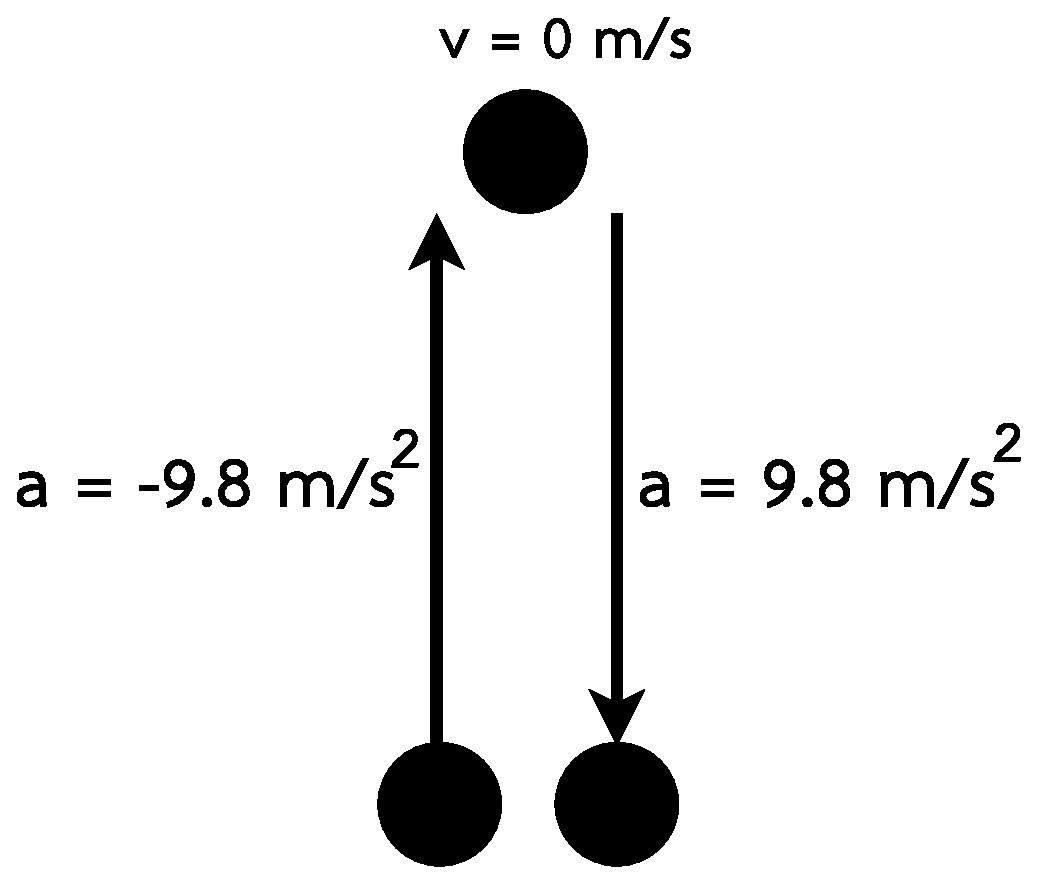
\includegraphics[width=\linewidth]{content-7.eps}
\end{minipage}
\end{adjustbox}
\end{c2}
\begin{enumerate}
\item \runningj \nonet ถ้าปล่อยให้วัตถุตกลงในแนวดิ่งอย่างเสรี    หากวัตถุนั้นตกกระทบพื้นดินในเวลา  10  วินาที   ถามว่าวัตถุกระทบดินด้วยความเร็วเท่ากับกี่เมตร/วินาที
\begin{4c}
	{4.9 m/s}{9.8 m/s}{49 m/s}{98 m/s}
\end{4c}
\end{enumerate}

\begin{enumerate}
\item \runningj \cmu{51} เมื่อโยนก้อนหินขึ้นไปในแนวดิ่งด้วยความเร็ว   4.9  เมตรต่อวินาที   ใช้เวลานานกี่วินาทีก้อนหินจึงจะมีความเร็วเป็นศูนย์
\begin{4c}
	{0.5}{1.0}{2.0}{4.0}
\end{4c}
\end{enumerate}

\section{การเคลื่อนที่แบบโปรเจกไทล์}
\begin{c2}\begin{wrapfigure}{r}{0.5\textwidth}
  \vspace{-20pt}
  \begin{center}
    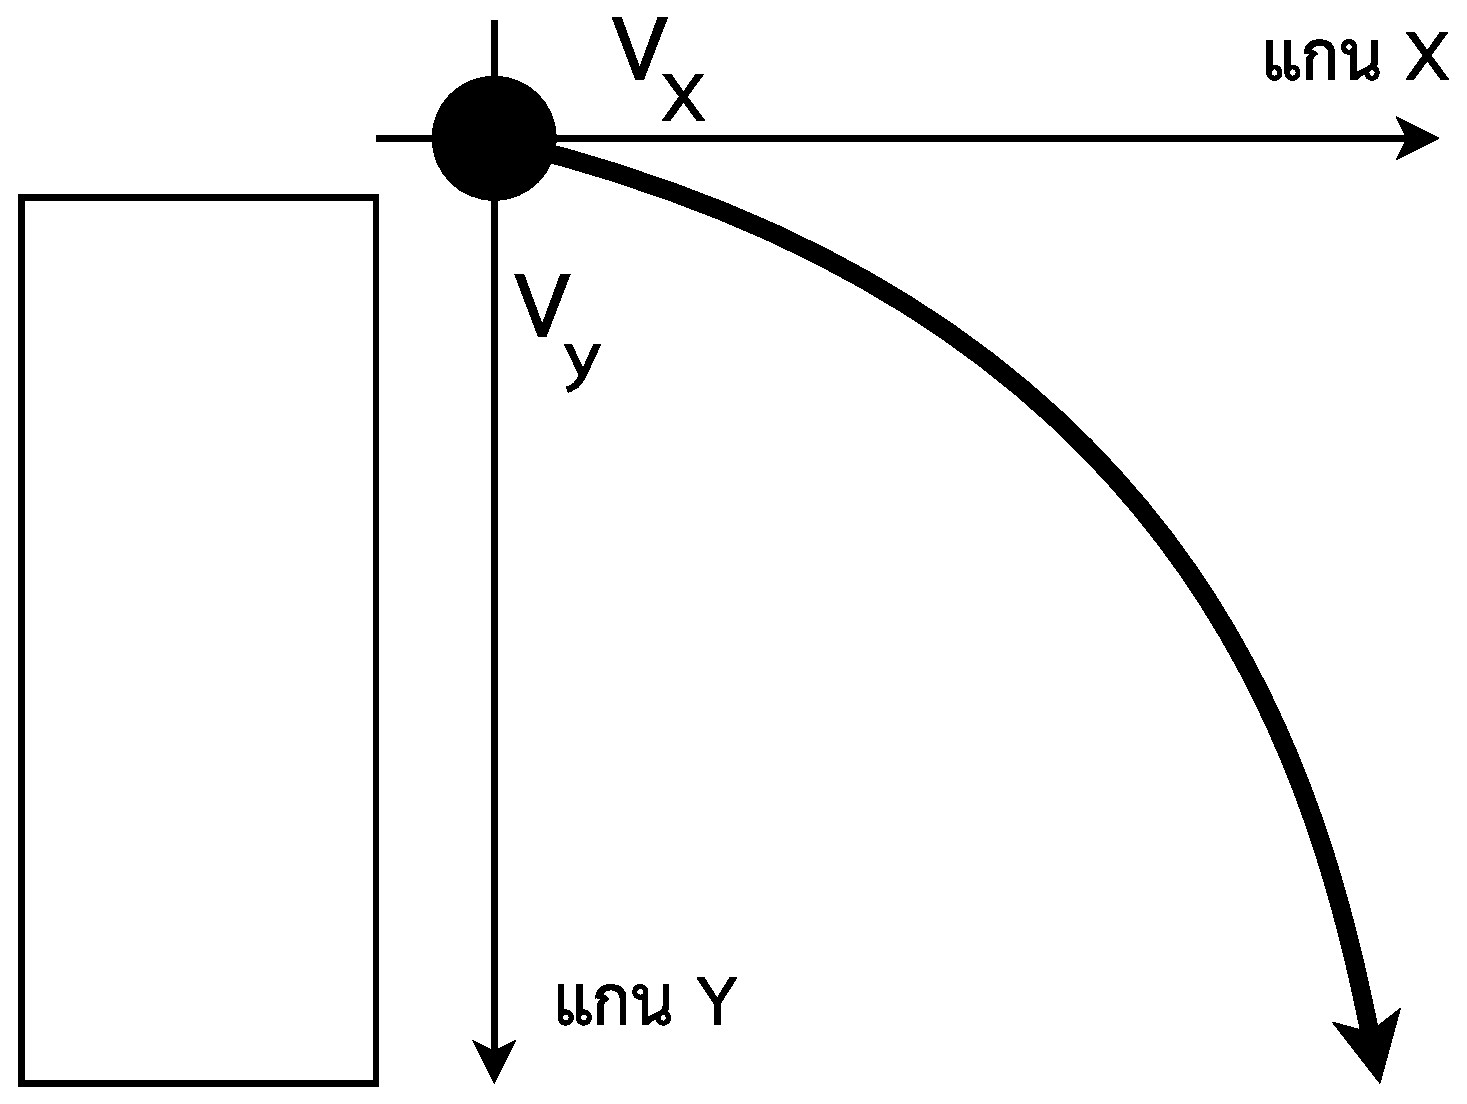
\includegraphics[width=0.4\textwidth]{content-8.eps}
  \end{center}
  \vspace{-20pt}
  \vspace{-10pt}
\end{wrapfigure}
\textbf{การเคลื่อนที่แบบโพรเจกไทล์}  คือ การเคลื่อนที่ในแนวโค้งรูปพาราโบลา  เกิดจากการเคลื่อนที่หลายมิติผสมกัน  ตัวอย่างเช่นหากเราขว้างวัตถุออกไปในแนวระดับจากดาดฟ้าตึกแห่งหนึ่ง  เราจะพบว่าวัตถุจะมีความพยายามที่จะเคลื่อนที่ไปในแนวระดับ (แกน X) ตามแรงที่เราขว้าง  พร้อมกันนั้นวัตถุจะถูกแรงโน้มถ่วงของโลก  ดึงให้เคลื่อนที่ตกลงมาในแนวดิ่ง (แกน Y) ด้วย    และเนื่องจากการเคลื่อนที่ทั้งสองแนวนี้เกิดในเวลาเดียวกัน      จึงเกิดการผสมผสานกันกลายเป็นการเคลื่อนที่แบบเส้นโค้งพาราโบลาพุ่งออกมาระหว่างกลางแนวระดับ (แกน X)  และแนวดิ่ง (แกน Y) ดังรูป  การเคลื่อนที่ในวิถีโค้งแบบนี้เรียกว่าเป็น \textbf{การเคลื่อนที่แบบโพรเจกไทล์}
\end{c2}
\begin{enumerate}
\item \runningj \nonet ข้อใดใกล้เคียงกับการเคลื่อนที่แบบโพรเจกไทล์มากที่สุด
\begin{2c}
	{เครื่องบินขณะบินขึ้นจากสนามบิน}{เด็กเล่นไม้ลื่น}
	{ลูกเทนนิสที่ถูกตีออกไปข้างหน้า}{เครื่องร่อนขณะร่อนลง}
\end{2c}
\end{enumerate}

\begin{c2}\centering{\textbf{ข้อควรรู้เบื้องต้นเกี่ยวกับการเคลื่อนที่แบบโพรเจกไทล์}}
\tcblower
\begin{minipage}{.6\textwidth}
	\begin{itemize}[leftmargin=*]
		\item[1)] อัตราเร็วของการเคลื่อนที่ในแนวระดับ (แกน X) ($v_x$) จะมีค่าคงที่ แต่ในแนวดิ่ง (แกน Y)($v_y$) วัตถุจะมีความเร่งเนื่องจากแรงโน้มถ่วง ( g )   คงตัวอยู่ตลอดเวลา    จึงทำให้ความเร็วในดิ่งมีค่าเปลี่ยนแปลงอยู่ตลอดเวลา
	\end{itemize}
\end{minipage}
\hfill
\begin{adjustbox}{valign=c} 
	\begin{minipage}[t]{.35\linewidth}
		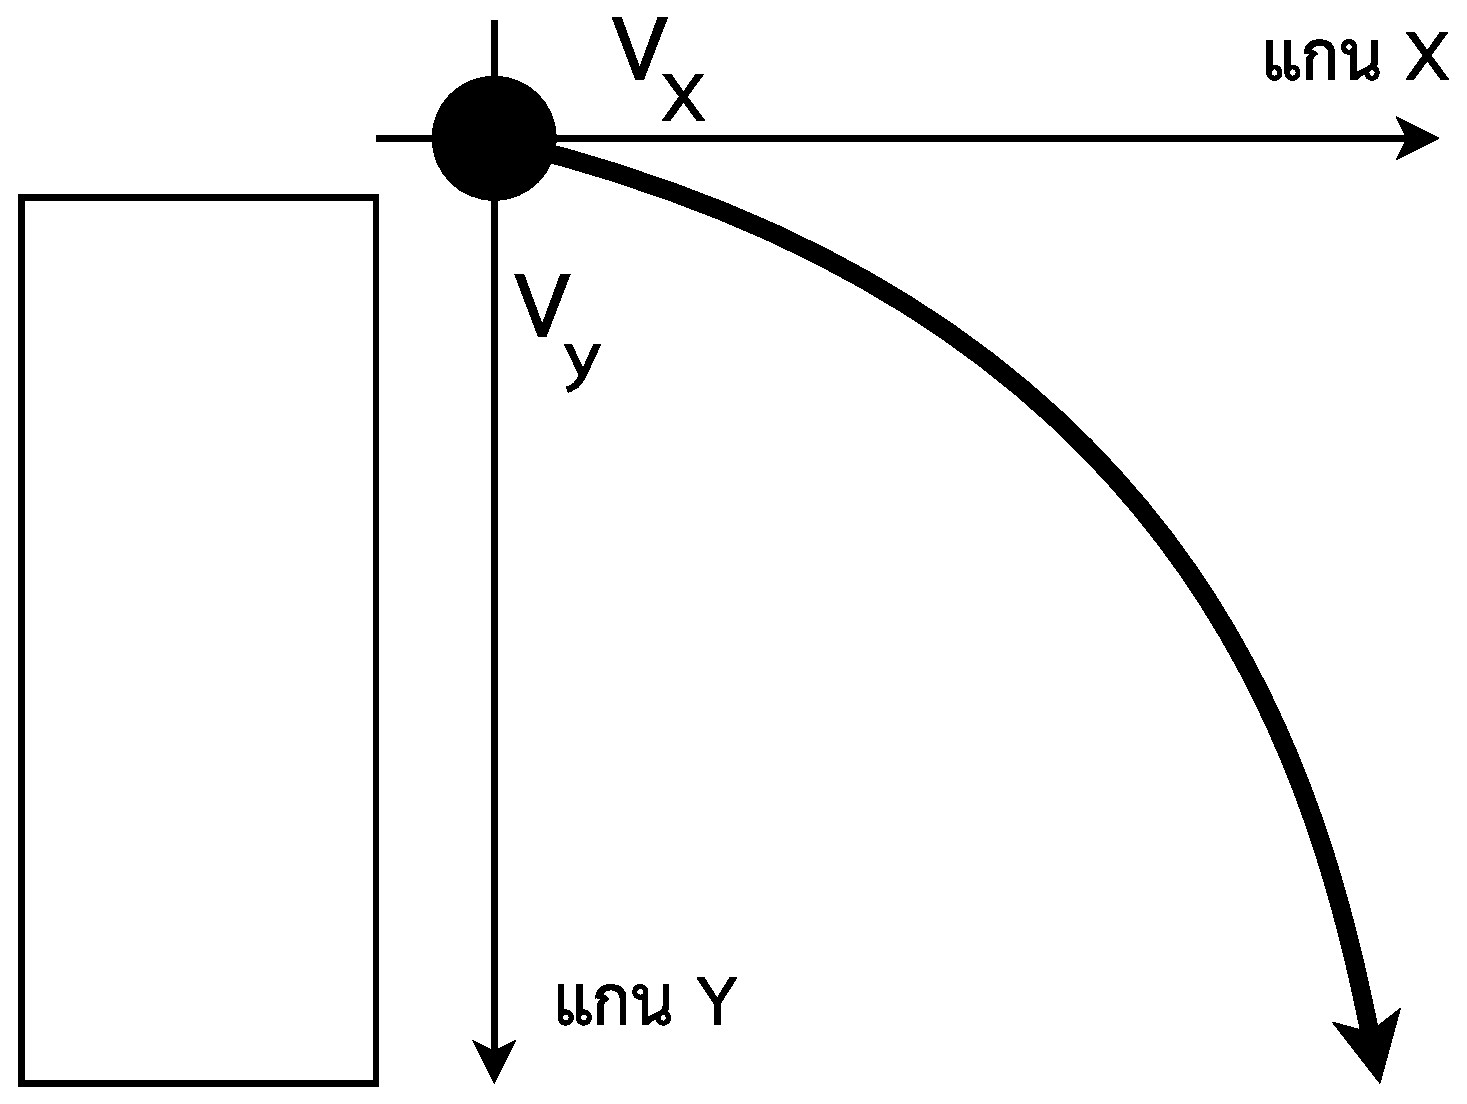
\includegraphics[width=\linewidth]{content-9-1.eps}
	\end{minipage}
\end{adjustbox}

\begin{minipage}{.6\textwidth}
	\begin{itemize}[leftmargin=*]
		\item[2)] พิจารณาการเคลื่อนที่แบบโพรเจกไทล์ชนิดโยนวัตถุจากพื้นขึ้นไปบนอากาศแล้วให้โค้งตกลงมา หากต้องการให้วัตถุเคลื่อนที่ไปในแนวระดับได้ไกลที่สุดต้องโยนวัตถุขึ้นไปในแนวเอียงทำมุม  45$^o$  กับแนวระดับ     และที่จุดสูงสุดของการเคลื่อนที่    ความเร็วของแนวดิ่ง (แกน Y) $(v_y)$ จะมีค่าเป็นศูนย์เหลือแต่ความเร็วในแนวระดับ (แกน X) $(v_x)$   เท่ากับความเร็วแนวระดับของตอนเริ่มต้น     เพราะความเร็วแนวระดับจะคงที่   ทุก ๆ จุดของการเคลื่อนที่จะมีค่าเท่ากันตลอดเวลา
	\end{itemize}
\end{minipage}
\hfill
\begin{adjustbox}{valign=c} 
	\begin{minipage}[t]{.35\linewidth}
		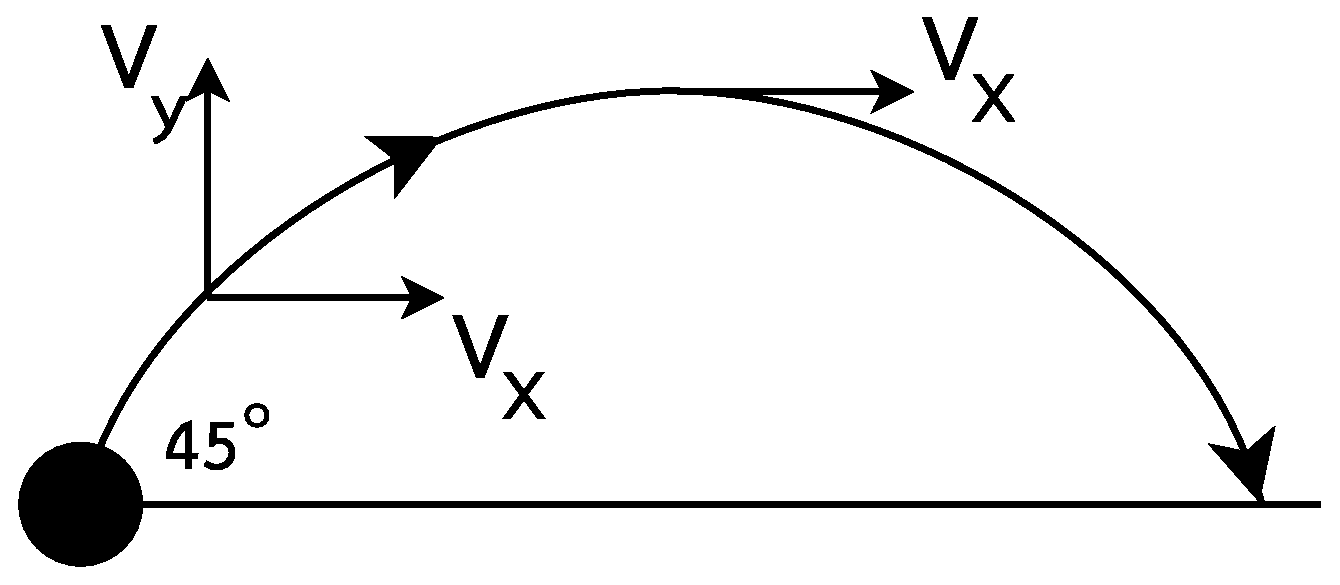
\includegraphics[width=\linewidth]{content-9-2.eps}
	\end{minipage}
\end{adjustbox}

\end{c2}
\begin{enumerate}
	\item \runningj \nonet ยิงลูกปืนออกไปในแนวระดับทําให้ลูกปืนเคลื่อนที่แบบโพรเจกไทล์   ตอนที่ลูกปืนกําลังจะกระทบพื้น  ข้อใด\textbf{ถูกต้องที่สุด}   (ไม่ต้องคิดแรงต้านอากาศ)
	\begin{1c}
		{ความเร็วในแนวระดับเป็นศูนย์}
		{ความเร็วในแนวระดับมีขนาดมากกว่าตอนที่ถูกยิงออกมา }
		{ความเร็วในแนวระดับมีขนาดน้อยกว่าตอนที่ถูกยิงออกมาแต่ไม่เป็นศูนย์}
		{ความเร็วในแนวระดับเท่ากับความเร็วตอนต้นที่ลูกปืนถูกยิงออกมา}
	\end{1c}
\end{enumerate}

\section{การเคลื่อนที่แบบวงกลม}
\begin{c2}การเคลื่อนที่แบบวงกลม  เป็นการเคลื่อนที่ในแนวโค้งรอบจุดศูนย์กลางจุดหนึ่ง   เช่นการเคลื่อนที่ของวัตถุที่ผูกไว้ด้วยเชือกแล้วเหวี่ยงให้เคลื่อนที่เป็นวงกลม   ,   การเคลื่อนที่ของรถไฟเหาะตีลังกา  ,   การเลี้ยวโค้งบนถนนของรถ   หรือการโคจรของดวงจันทร์รอบโลก  เป็นต้น
\begin{center}
\begin{minipage}{.45\textwidth}
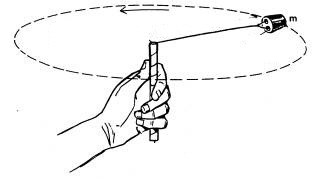
\includegraphics[width=\textwidth]{content-10-1.jpg}
\end{minipage} \hfill
\begin{minipage}{.45\textwidth}
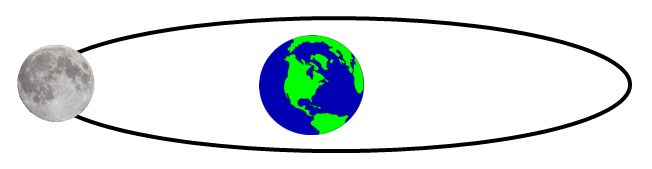
\includegraphics[width=\textwidth]{content-10-2.jpg}
\end{minipage}
\end{center}
\begin{center}
\begin{minipage}{.45\textwidth}
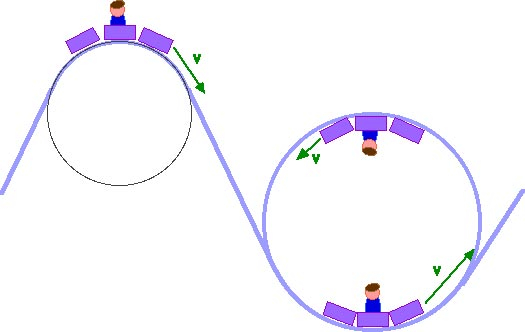
\includegraphics[width=\textwidth]{content-10-3.jpg}
\end{minipage} \hfill
\begin{minipage}{.45\textwidth}
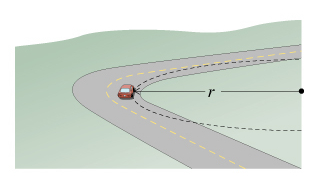
\includegraphics[width=\textwidth]{content-10-4.jpg}
\end{minipage}
\end{center}
\end{c2}
\begin{enumerate}
	\item \runningj \cmu{49} การเคลื่อนที่ในข้อใดไม่เป็นการเคลื่อนที่แบบโพรเจกไทล์
	\begin{2c}
		{ชู้ตลูกบาสเก็ตบอลลงห่วง}{ขว้างก้อนหินในแนวระดับ}
		{ยิงลูกธนูเข้าเป้าตาวัว}{ขับรถยนต์เข้าโค้ง}
	\end{2c}
\end{enumerate}

\begin{c2}\centering{\textbf{ก่อนศึกษารายละเอียดเกี่ยวกับการเคลื่อนที่แบบวงกลม นักเรียนต้องทำความเข้าใจคำศัพท์ต่อไปนี้ให้ดีก่อน}}
\tcblower
\begin{minipage}{.6\textwidth}
	\begin{itemize}[leftmargin=*]
		\item[1)] คาบ (T)  คือเวลาที่ใช้ในการเคลื่อนที่ครบ  1 รอบ มีหน่วยเป็นวินาที (s)
		\item[2)] ความถี่ (f)  คือจำนวนรอบที่เคลื่อนที่ได้ในหนึ่งหน่วยเวลามีหน่วยเป็น  รอบ/วินาที  หรือเฮิรตซ์ (Hz)  เราสามารถหาค่าความถี่ได้จากสมการต่อไปนี้ \\
				  $$f = \frac{\text{จำนวนรอบ}}{\text{เวลา}} \quad \text{หรือ} \quad f = \frac{1}{T}$$
				\begin{tabbing}
					\textbf{เมื่อ} \quad 	\=f \quad\=\textbf{คือ}ความถี่ (Hz) \\
										\>T \>\textbf{คือ}คาบของการเคลื่อนที่ (วินาที)
				\end{tabbing}
	\end{itemize}
\end{minipage}
\hfill
\begin{adjustbox}{valign=c} 
    \begin{minipage}[t]{.35\linewidth}
        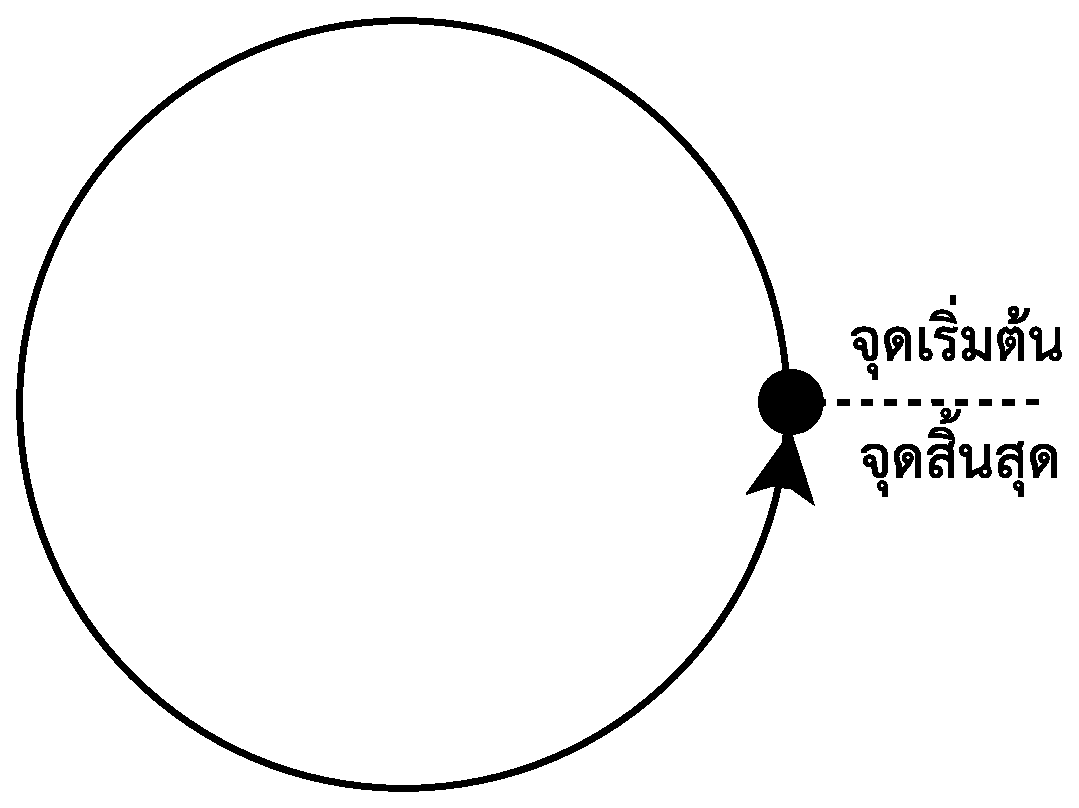
\includegraphics[width=\linewidth]{content-11.eps}
    \end{minipage}
\end{adjustbox}
\end{c2}
\begin{enumerate}
	\item \runningj \nonet เหวี่ยงจุกยางให้เคลื่อนที่เป็นแนววงกลมในระนาบระดับศีรษะ  10  รอบ  ใช้เวลา  4  วินาที   จุกยางเคลื่อนที่ด้วยความถี่เท่าใด
	\begin{2c}
		{0.25  รอบ/วินาที}{0.5  รอบ/วินาที	}
		{2.5  รอบ/วินาที}{5.0  รอบ/วินาที}
	\end{2c}
\end{enumerate}

\begin{c2}\begin{minipage}{.65\textwidth}
โดยทั่วไปแล้วการเคลื่อนที่แบบวงกลม จะมีแรงเกี่ยวข้องอย่างน้อย  2  แรงเสมอ  ได้แก่
\begin{itemize}[leftmargin=*]
	\item[1)] \textbf{แรงหนีศูนย์กลาง}  จะพยายามผลักวัตถุออกไปจาก\\วงกลมอยู่ตลอดเวลา
	\item[2)] \textbf{แรงเข้าสู่ศูนย์กลาง}   จะพยายามดึงวัตถุเข้าสู่จุด\\ศูนย์กลางของวงกลมเสมอ	
\end{itemize}
\end{minipage} \hfill
\begin{adjustbox}{valign=c} 
    \begin{minipage}[c]{.3\linewidth}
        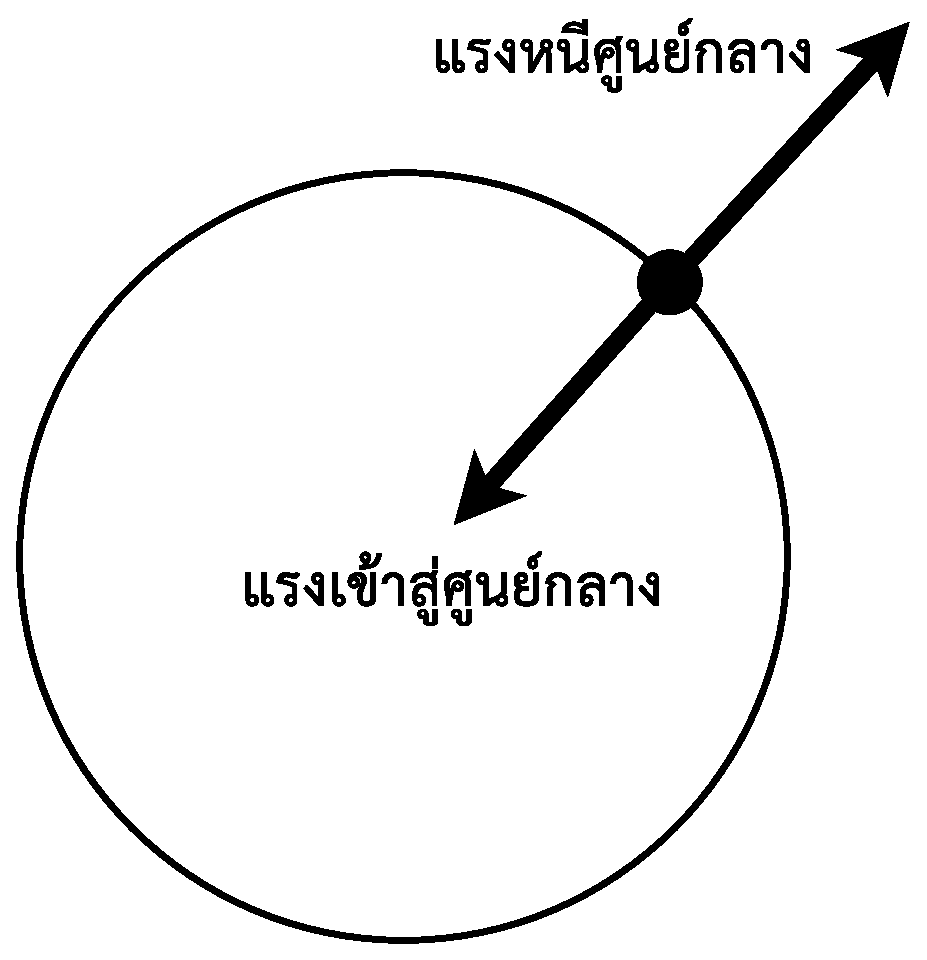
\includegraphics[width=\linewidth]{content-12.eps}
    \end{minipage}
\end{adjustbox}
\tcblower
ปกติแล้วแรงทั้งสองนี้จะมีขนาดเท่ากัน แต่มีทิศตรงกันข้ามดังรูป   ทั้งนี้เพื่อให้วัตถุอยู่ในภาวะสมดุลของแรงนั่นเอง แรงเข้าสู่ศูนย์กลางของการเคลื่อนที่แต่กรณีอาจมีลักษณะที่แตกต่างกันไป   \textbf{ตัวอย่างเช่น}
\begin{center}
\begin{minipage}{.6\textwidth}
การเคลื่อนที่ของวัตถุที่ผูกไว้ด้วยเชือกแล้วเหวี่ยงให้เคลื่อนที่เป็นวงกลม       แรงที่ทำหน้าที่เป็นแรงเข้าสู่ศูนย์กลางคือแรงดึงเชือก
\end{minipage} \hfill
\begin{adjustbox}{valign=c} 
    \begin{minipage}[t]{.35\linewidth}
        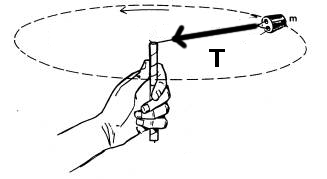
\includegraphics[width=\linewidth]{content-12-1.jpg}
    \end{minipage}
\end{adjustbox}
\end{center}

\begin{center}
\begin{minipage}{.6\textwidth}
การเลี้ยวโค้งบนถนนของรถ	แรงที่ทำหน้าที่เป็นแรงเข้าสู่ศูนย์กลางคือแรงเสียดทานระหว่างยางรถกับพื้นถนน
\end{minipage} \hfill
\begin{adjustbox}{valign=c} 
    \begin{minipage}[t]{.35\linewidth}
        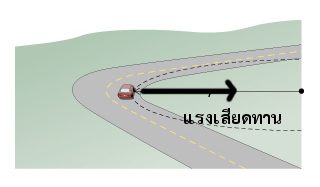
\includegraphics[width=\linewidth]{content-12-4.jpg}
    \end{minipage}
\end{adjustbox}
\end{center}

\begin{center}
\begin{minipage}{.6\textwidth}
การโคจรของดวงจันทร์รอบโลกแรงที่ทำหน้าที่เป็นแรงเข้าสู่ศูนย์กลางคือแรงดึงดูดที่โลกดูดดวงจันทร์ไว้นั่นเอง
\end{minipage} \hfill
\begin{adjustbox}{valign=c} 
    \begin{minipage}[t]{.35\linewidth}
        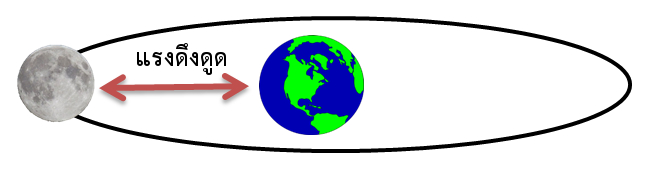
\includegraphics[width=\linewidth]{content-12-2.jpg}
    \end{minipage}
\end{adjustbox}
\end{center}

\begin{center}
\begin{minipage}{.6\textwidth}
การเคลื่อนที่ของรถไฟเหาะตีลังกา    หากรถอยู่ที่จุดสูงสุดของราง     แรงที่ทำหน้าที่เป็นแรงเข้าสู่ศูนย์กลางคือน้ำหนักรถไฟรวมกับแรงดันของพื้นราง    แต่ถ้ารถอยู่ที่จุดต่ำสุดของรางแรงที่ทำหน้าที่เป็นแรงเข้าสู่ศูนย์กลางคือน้ำหนักรถไฟอย่างเดียวดังแสดงในรูป
\end{minipage} \hfill
\begin{adjustbox}{valign=c} 
    \begin{minipage}[t]{.35\linewidth}
        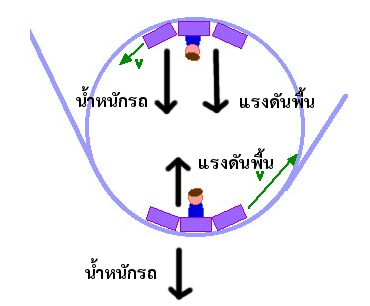
\includegraphics[width=\linewidth]{content-12-3.jpg}
    \end{minipage}
\end{adjustbox}
\end{center}
\end{c2}
\begin{enumerate}
	\item \runningj \nonet ผูกเชือกเข้ากับจุกยางแล้วเหวี่ยงให้จุกยางเคลื่อนที่เป็นวงกลมในแนวระดับเหนือศีรษะด้วยอัตราเร็วคงตัว  ข้อใดถูกต้อง
	\begin{1c}
		{แรงที่กระทําต่อจุกยางมีทิศเข้าสู่ศูนย์กลางวงกลม }
		{แรงที่กระทําต่อจุกยางมีทิศเดียวกับความเร็วของจุกยาง}
		{จุกยางมีความเร็วคงตัว}
		{จุกยางมีความเร่งเป็นศูนย์}
	\end{1c}
\end{enumerate}

\section{การเคลื่อนที่แบบฮาร์มอนิกอย่างง่าย}
\begin{c2}\textbf{การเคลื่อนที่แบบฮาร์มอนิกอย่างง่าย}  คือการเคลื่อนที่ซึ่งเคลื่อนที่กลับไปมาซ้ำทางเดิม  โดยผ่านตำแหน่งสมดุลโดยมีคาบของการเคลื่อนที่คงตัว   ตัวอย่างเช่นการสั้นของสปริง   การแกว่งของลูกตุ้มนาฬิกาหรือชิงช้า  เป็นต้น \\
\begin{center}
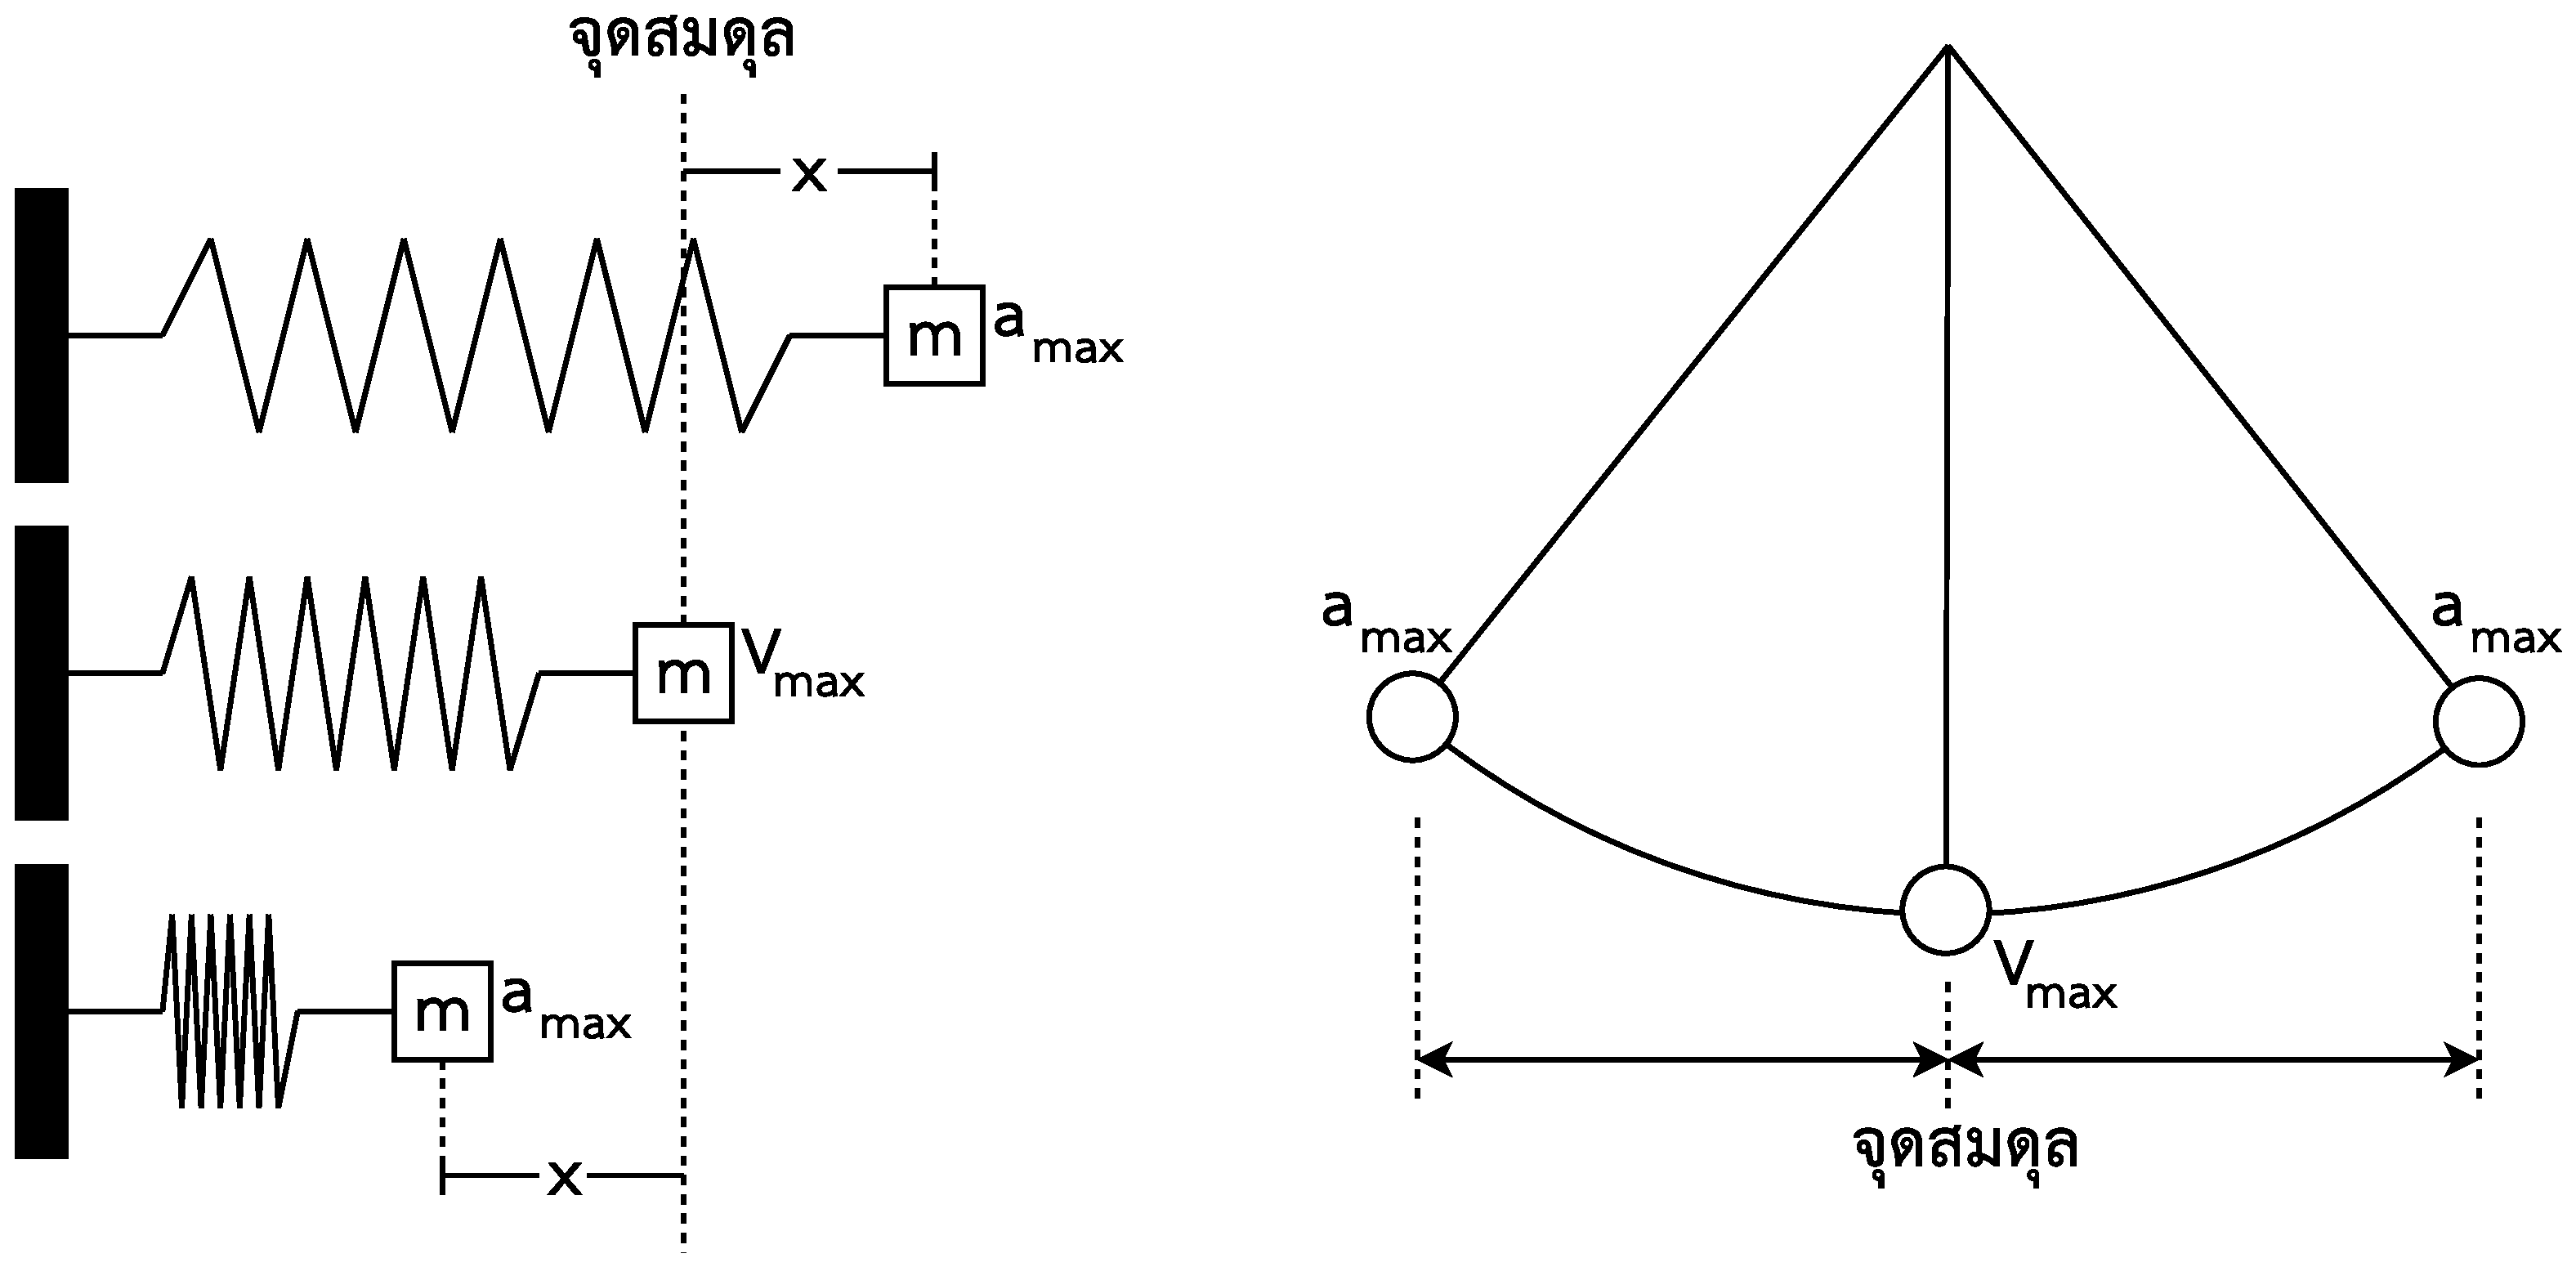
\includegraphics[width=\textwidth]{content-13.eps}
\end{center}
\end{c2}
\begin{enumerate}
	\item \runningj \nonet ข้อใดต่อไปนี้ไม่ได้ทำให้วัตถุมีการเคลื่อนที่แบบฮาร์มอนิกอย่างง่าย
	\begin{1c}
		{แขวนลูกตุ้มด้วยเชือกในแนวดิ่ง    ดึงลูกตุ้มออกมาจนเชือกทำมุมกับแนวดิ่งเล็กน้อยแล้วปล่อยมือ}
		{ผูกวัตถุกับปลายสปริงในแนวระดับ  ตรึงอีกด้านของสปริงไว้  ดึงวัตถุให้สปริงยืดออกเล็กน้อยแล้วปล่อยมือ}
		{ผูกวัตถุกับปลายสปริงในแนวดิ่ง   ตรึงอีกด้านของสปริงไว้  ดึงวัตถุให้สปริงยืดออกเล็กน้อยแล้วปล่อยมือ}
		{แขวนลูกตุ้มด้วยเชือกในแนวดิ่ง  ผลักลูกตุ้มให้แกว่งเป็นวงกลมในแนวราบ   โดยเส้นเชือกทำมุมคงตัวกับแนวดิ่ง}
	\end{1c}
\end{enumerate}

\begin{c2}\centering{\textbf{ข้อควรรู้เกี่ยวกับการเคลื่อนที่แบบฮาร์มอนิกอย่างง่าย}}
\tcblower
\begin{itemize}[leftmargin=*]
	\item[1)] 	\textbf{ขณะที่วัตถุกำลังเคลื่อนที่ผ่านจุดสมดุล (จุดตรงกลาง)}  วัตถุจะมีความเร็วสูงสุด $(v_{max})$  แต่มีความเร่ง (a)  ต่ำที่สุด \\
				\textbf{ขณะที่วัตถุอยู่ที่จุดตรงปลายของการเคลื่อนที่}  วัตถุจะมีความเร่งสูงสุด $(a_{max})$  แต่มีความเร็ว (v) ต่ำที่สุด	
	\item[2)] 	\adjustbox{valign=t}{
					\begin{minipage}{.6\linewidth}
						คาบ (T)  คือเวลาที่ใช้ในการเคลื่อนที่ครบ  1  รอบ มีหน่วยเป็นวินาที (s)\\\\
						สำหรับคาบของการเคลื่อนที่ฮาร์มอนิกอย่างง่ายแบบแกว่ง  เราสามารถหาคาบของการแกว่งได้จากสมการ
						\[ T=2\pi\sqrt{\frac{L}{g}}\]
					\end{minipage}} \hfill
				\adjustbox{valign=t}{
					\begin{minipage}{.35\linewidth}
						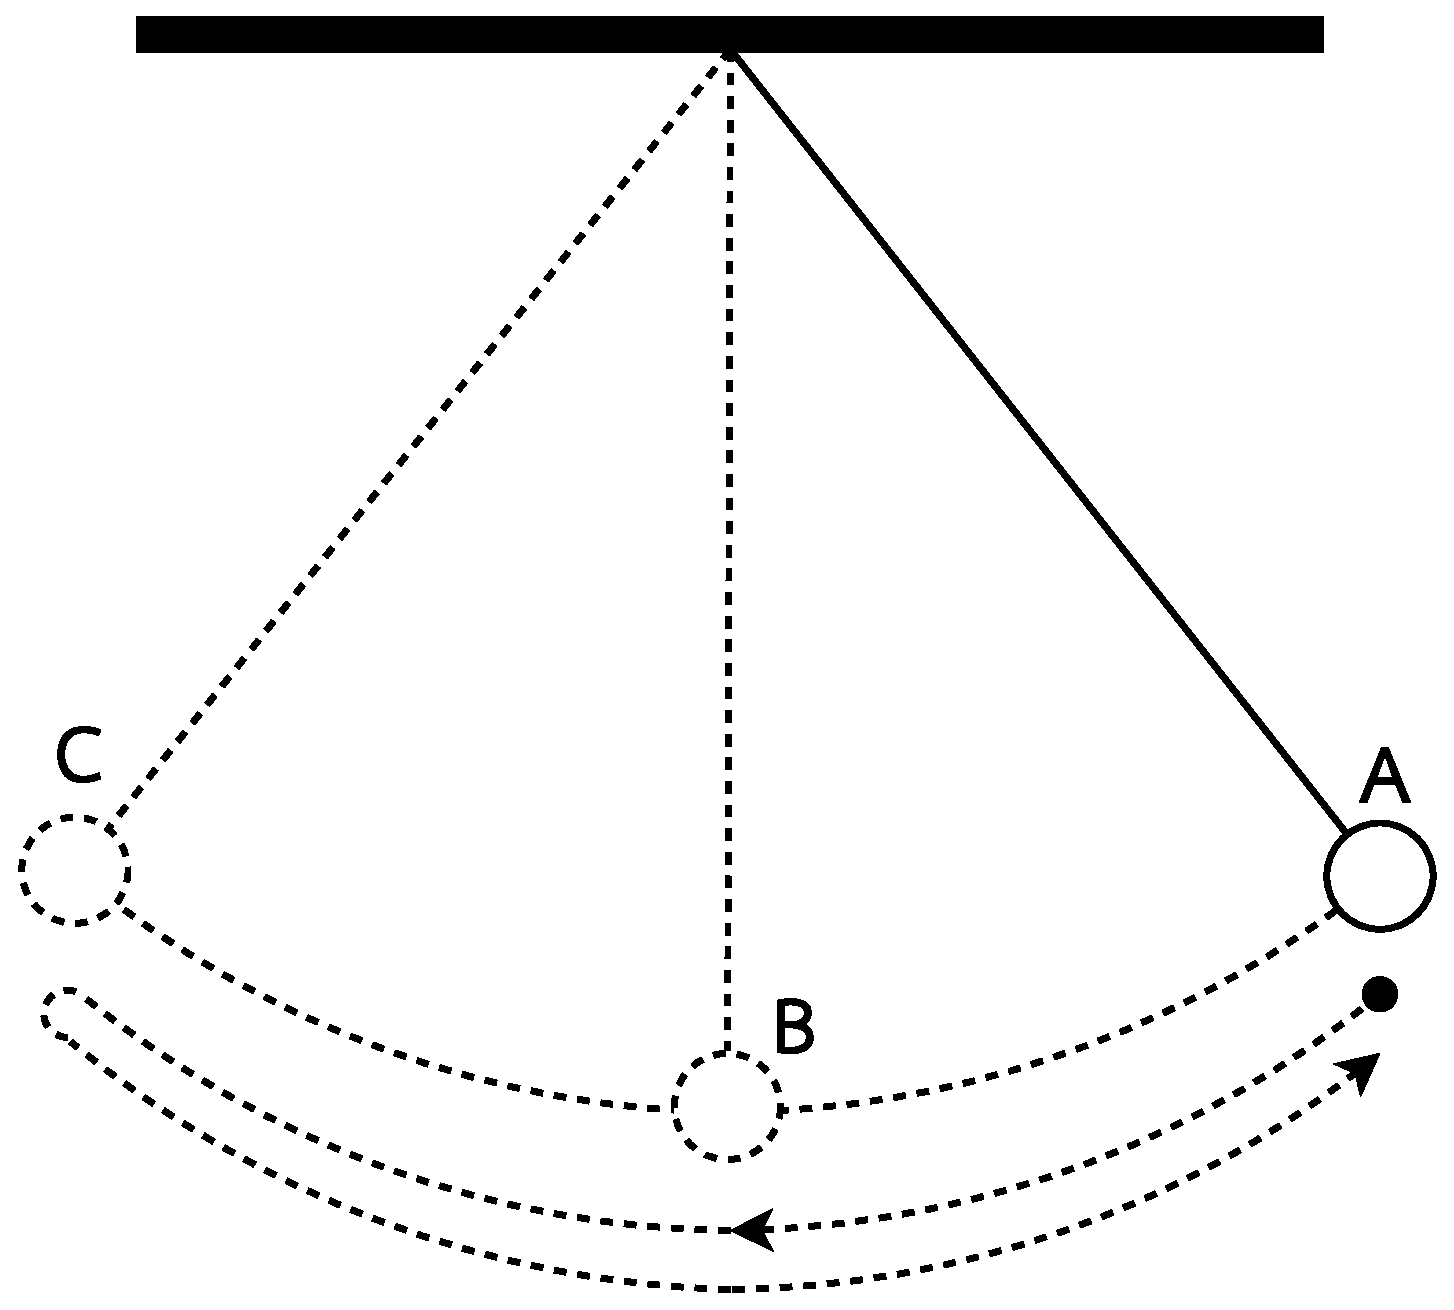
\includegraphics[width=\textwidth]{content-14.eps}
					\end{minipage}
				}
				\begin{tabbing}
					\textbf{เมื่อ} \quad 	\=T \quad 	\=\textbf{คือ} 	\=คาบของการแกว่ง  มีหน่วยเป็น วินาที (s) \\
										\>L 		\>\textbf{คือ} 	\>คือระยะจากจุดตรึงสายแกว่งถึงจุดศูนย์กลางลูกตุ้ม มีหน่วยเป็น \\
										\>			\>				\>เมตร (m)\\
										\>g			\>\textbf{คือ} 	\>คือความเร่งเนื่องจากแรงโน้มถ่วง มีหน่วยเป็น เมตร/วินาที$^2$ ($m/s^2$)
				\end{tabbing}
	\item[3)] 	ความถี่ (f)  คือจำนวนรอบที่เคลื่อนที่ได้ในหนึ่งหน่วยเวลา  มีหน่วยเป็น  รอบ/วินาที หรือเฮิรตซ์ (Hz) เราสามารถหาค่าความถี่ได้จากสมการต่อไปนี้\\
				\[ f = \frac{\text{จำนวนรอบ}}{\text{เวลา}} \qquad	\text{หรือ}	\qquad	f = \frac{1}{T}\]
				\begin{tabbing}
					\textbf{เมื่อ} \quad 	\=f \quad 	\=\textbf{คือ} 	\=ความถี่ (Hz)\\
										\>T 		\>\textbf{คือ} 	\>คาบของการเคลื่อนที่  (วินาที)
				\end{tabbing}
\end{itemize}
\end{c2}
\begin{enumerate}
	\item \runningj \nonet ลูกตุ้มนาฬิกากำลังแกว่งกลับไปกลับมาแบบฮาร์มอนิกอย่างง่าย   ที่ตำแหน่งสมดุลของการแกว่งลูกตุ้มนาฬิกามีสภาพการเคลื่อนที่เป็นอย่างไร
	\begin{2c}
		{ความเร็วสูงสุด  ความเร่งต่ำสุด}{ความเร็วต่ำสุด  ความเร่งต่ำสุด}
		{ความเร็วสูงสุด  ความเร่งสูงสุด}{ความเร็วต่ำสุด  ความเร่งสูงสุด}
	\end{2c}
\end{enumerate}



\end{document}
